\chapter{HAWK -- Hybrid Question Answering using Linked Data}


\graffito{
HAWK has been developed to bridge the gap between unstructured and structured knowledge bases in question answering. 
The approach is published in~\cite{HAWK_CLEF_2015,HAWK_NLIWOD_2015,hawk_2015}.
HAWK won the 2nd price at the \ac{QALD} challenge, task 2 2015.
}

Recent advances in \ac{QA} over \ac{LD} provide end users with more and more sophisticated tools for querying \ac{LD} by allowing users to express their information need in natural language~\cite{SINA_WebSemantic,pythia,template}. 
This allows access to the wealth of semantic data available on the Semantic Web also to non-experts and users unaware of the underlying schema. 
Linked Data eases the access to structured and semantic meaningful information than unstructured web documents.
However, a lot of information is still available only in textual form, both on the Document Web and in the form of labels and abstracts in \ac{LD} sources~\cite{GER+13}.
Therefore, a considerable number of questions can only be answered by using hybrid question answering approaches, which  can find and combine information stored in both structured and textual data sources~\cite{combiningLDandIR}.

In this chapter, we present HAWK, the (to best of our knowledge) first full-fledged hybrid \ac{QA} framework for entity search over \ac{LD} and textual data. 
%To the best of our knowledge, this is the first hybrid question answering system, combining information from structured and unstructured data.
Given a textual input query $q$, HAWK implements a 13-step pipeline, which comprises 1) input segmentation 2) part-of-speech tagging, 3) detecting entities, 4) spotting noun phrases, 5) dependency parsing and 6) applying linguistic pruning heuristics for an in-depth analysis of the natural language input. 
The results of these first six steps is a predicate-argument graph annotated with resources from the Linked Data Web. HAWK then 7) assigns semantic meaning to nodes and 8) generates basic triple patterns for each component of the input query with respect to a multitude of features. 
This deductive linking of triples results in a set of SPARQL queries containing text operators as well as triple patterns.
In order to reduce operational costs, 9) HAWK discards queries using several rules, e.g., by  discarding not connected query graphs.
10) HAWK uses a prefix-based classifier to decide whether it is boolean question and depending on the result 11) modifies the SPARQL query or 12) calculated the query modifiers.
Finally, 13) queries are ranked using extensible feature vectors and cosine similarity.

%%We evaluate HAWK on the \ac{QALD}-4 benchmark\footnote{\url{http://www.sc.cit-ec.uni-bielefeld.de/qald/}} for hybrid question answering. 
%As data source it uses a triple store containing DBpedia 3.9 as well as full-text information based on the Wikipedia abstracts of all loaded resources.
%The evaluation sections reports on micro F-measure, and analyzes the influence of different entity annotation systems on the overall question answering performance.

%\todo[inline]{@Axel: Contribs}
Our main contributions can be summarized as follows:
 \begin{itemize}
 \item We present the first \ac{QA} framework for answering hybrid questions;
 \item HAWK analyses input queries based on predicate-argument trees to deeply understand and match semantic resources;
 \item Our framework is generic as it does not rely on templates. It is thus inherently able to cover a wide variety of natural language questions. % as well as knowledge bases with various topologies;
 \item The modular architecture of HAWK allows simple exchanging of pipeline parts to enhance testing and deployment;
 %\item HAWK's implementation is open-source under MIT License\footnote{\url{https://github.com/AKSW/hawk}};
 \item Our evaluation suggests that HAWK is able to achieve F-measures of 0.61 on rather small training datasets.
 \item We present a thorough evaluation of the framework, including an analysis of the influence of entity annotation tools on the generation process of the hybrid queries and a study of the overall accuracy of the system. 
 \item Furthermore, HAWK can generate SPARQL queries using \texttt{ASK}. Our results show that these developments lead to HAWK achieving 0.74 F-measure on the ASK queries contained in the Question Answering over Linked Data (\ac{QALD}-5) hybrid query benchmark~\cite{qald5} assuming an given optimal ranking function.
 \end{itemize}

The remaining chapter is structured as follows:
We explain HAWK's methodology in detail in Section~\ref{chahawk:sec:method} and illustrate the pipeline steps on several examples in Section~\ref{sec:hawkexample}.
HAWK's performance and the influence of entity annotation systems is evaluated in Section~\ref{chahawk:sec:evaluation}. 
%Section~\ref{chahawk:sec:relatedwork} discusses related work.  
%Finally, we conclude in Section~\ref{chahawk:sec:conclusion}. 
Additional information can be found at our project home page \url{http://aksw.org/Projects/HAWK.html}.

\section{Method}
\label{chahawk:sec:method}

In the following, we describe the architecture and methodology of HAWK. 
Figure~\ref{fig:hawk_pipeline} gives an overview of the architecture of HAWK. In the following we describe the depicted steps in more detail.%: POS-tagging, entity annotation, dependency parsing, linguistic pruning, semantic annotation, SPARQL query generation, pruning and ranking.

\begin{figure}[tb!]
\centering
\usetikzlibrary{positioning,shapes,arrows}
% Define block styles
\tikzstyle{decision} = [diamond, draw, fill=blue!20, 
    text width=5em, text badly centered, node distance=3cm, inner sep=0pt]
\tikzstyle{block} = [rectangle, draw, fill=blue!20, 
    text width=5.5em, text centered, rounded corners, minimum height=4em]
\tikzstyle{line} = [draw, -latex']
\tikzstyle{cloud} = [draw, ellipse,fill=red!20, node distance=3cm,
    minimum height=2em]

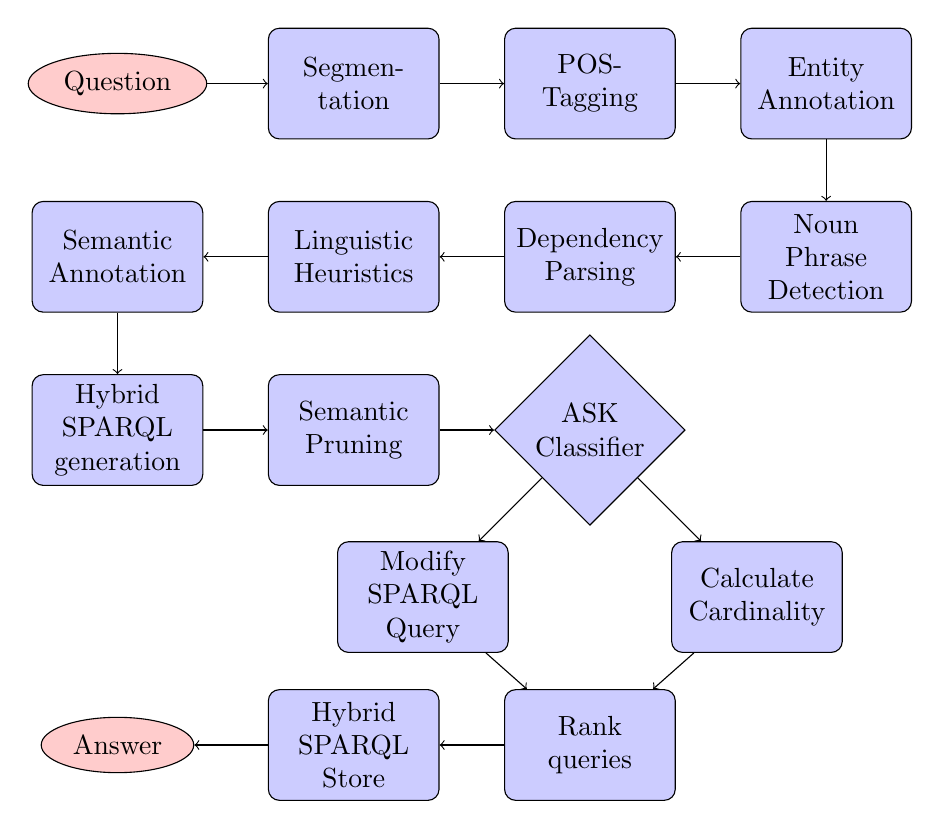
\begin{tikzpicture}[->,node distance = 3cm, auto]
    % Place nodes
    \node [cloud] (question) {Question};
    \node [block, right of=question] (segmentation) {Segmen\-tation};
    \node [block, right of=segmentation] (pos) {POS-Tagging};
    \node [block, right of=pos] (entityannotation) {Entity Annotation};
    \node [block, below of=entityannotation, node distance=2.2cm] (nounphrasedetection) {Noun Phrase Detection};
    \node [block, left of=nounphrasedetection] (dependency) {Dependency Parsing};
    \node [block, left of=dependency] (ling_heu) {Linguistic Heuristics};
    \node [block, left of=ling_heu] (sem_anno) {Semantic Annotation};
    \node [block, below of=sem_anno,node distance=2.2cm] (sparql) {Hybrid SPARQL generation};
    \node [block, right of=sparql] (sem_pruning) {Semantic Pruning};
    \node [decision, right of=sem_pruning] (classify) {ASK Classifier};
    \node [block, below left of=classify] (mod_ask) {Modify SPARQL Query};
    \node [block, below right of=classify] (calc_card) {Calculate Cardinality};
    \node [block, below of=classify,  node distance=4cm] (rank) {Rank queries};
    \node [block, left of=rank] (sparql_fire) {Hybrid SPARQL Store};
    \node [cloud, left of=sparql_fire] (answer) {Answer};
    %\node [decision, below of=evaluate] (decide) {is best candidate better?};
    % Draw edges
    \draw[->]  (question) -- (segmentation);
    \draw[->]  (segmentation) -- (pos);
    \draw[->]  (pos) -- (entityannotation);
    \draw[->]  (entityannotation) -- (nounphrasedetection);
    \draw[->]  (nounphrasedetection) -- (dependency);
    \draw[->]  (dependency) -- (ling_heu);
    \draw[->]  (ling_heu) -- (sem_anno);
    \draw[->]  (sem_anno) -- (sparql);
    \draw[->]  (sparql) -- (sem_pruning);
    \draw[->]  (sem_pruning) -- (classify);
    \draw[->]  (classify) -- (mod_ask);
    \draw[->]  (classify) -- (calc_card);
    \draw[->]  (mod_ask) -- (rank);
    \draw[->]  (calc_card) -- (rank);
    \draw[->]  (rank) -- (sparql_fire);
    \draw[->]  (sparql_fire) -- (answer);


   % \path [line] (decide) -| node [near start] {yes} (update);
   % \path [line] (update) |- (identify);
   %    \path [line] (decide) -- node {no}(stop);
\end{tikzpicture}
\caption{Pipeline steps of HAWK.}
\label{fig:hawk_pipeline}
\end{figure}

\subsection{Input Segmentation.} 
To be generic with respect to the language of the input question, HAWK uses a modular system that is able of tokenizing even languages without clear separation like Chinese\footnote{\url{https://github.com/clir/clearnlp}}.
For English input questions our system relies on the \emph{clearNLP}-framework~\cite{choi2011getting} which provides a.o. a white space tokenizer, POS-tagger and transition-based dependency parsing.

\subsection{Part-of-Speech (POS)-Tagging.} 
HAWK annotates each token with its POS-tag which will be later used to identify possible semantic annotations. 
A large number of frameworks have been developed for these purposes over the last years. 
Currently, we rely on \emph{clearNLP}~\cite{choi2011getting} which is a fast and robust framework~\cite{choi-palmer:2012:ACL2012short}.

%\subsection{POS-Tagging, Segmentation}
%\todo[inline]{re is no tokenisation/segmentation component in the pipeline?}
%A large number of frameworks have been developed for these purposes over the last years. 
%We rely on \emph{clearNLP}~\cite{choi2011getting} which is based on transition-based dependency parsing and sophisticated segmentation algorithm.

\subsection{Entity Annotation}
HAWK identifies named entities and tries to link them to semantic entities from the underlying knowledge base, in our case DBpedia 2014\footnote{Status of May 2015. The dataset choice is influenced by the benchmark requirements.}, via well-established entity annotation tools, also called entity tagging tools:
\begin{itemize}
\item \textbf{Wikipedia Miner}~\cite{milne2008learning} is based on different facts like prior probabilities, context relatedness and quality, which are then combined and tuned using a classifier.
\item \textbf{DBpedia Spotlight}~\cite{spotlight} %, one of the first semantic entity annotation approaches, 
was published in 2011. 
This tool combines named entity recognition and disambiguation based on DBpedia.
\item \textbf{TagMe 2}~\cite{TagMe2} is based on a directory of links, pages and an inlink graph from Wikipedia.
The approach recognizes entities by matching terms with Wikipedia link texts and disambiguates the match using the in-link graph and the page dataset.
%Afterwards, TagMe 2 prunes identified named entities which are considered as non-coherent to the rest of the named entities in the input text.  
\item \textbf{FOX}~\cite{FOX} has been introduced 2014 as an ensemble learning-based approach combining several state-of-the-art named entity recognition approaches. 
The FOX framework outperforms the current state of the art entity recognizers and relies on the entity linking tool AGDISTIS~\cite{agdistis_iswc}.
\end{itemize}
Additionally, we implemented two artificial spotters for evaluation:
\begin{itemize}
\item \textbf{Union} is a spotter that combines the result sets of the above introduced spotters and returns thus a superset of all spotters.
\item \textbf{Optimal} will spot all entities from the gold standard to be able to ignore spotting influences in the following steps of the pipeline.
\end{itemize}

HAWK annotates the POS-tag \texttt{ADD} to these named entities to differentiate named entities from other tokens. % for our running example from above.
The influence of the entity annotation module is evaluated in Section~\ref{chahawk:sec:evaluation}.

\subsection{Noun Phrase Detection.}
HAWK identifies noun phrases, i.e., semantically meaningful word groups, e.g., real-world entities or concepts not captured by the underlying knowledge base or not yet recognized by the entity annotation system, using the result of the POS-tagging step. 
This step is also know as chunking. 
Input tokens are combined following manually-crafted linguistic heuristics based on POS-tag sequences derived from the \ac{QALD}-5 benchmark questions and their POS-tag is changed to \texttt{CNN} which we introduce to the system.
Two domain experts implemented the deduced POS-tag sequences and safeguarded the quality of this algorithm w.r.t. the \ac{QA} pipeline f-measure. 
The full algorithm can be found in Algorithm~\ref{listing:nouncombiner}.

\begin{algorithm}[tb!]
\SetAlgoLined
\KwData{Tokenized question ($list$) with Part-of-Speech-tags (POS-tags)}
	subsequence = ()\;
	\For{$t \in [0,|list|]$ }{
			token = list.get($t$)\;
			%// look for start "RB|JJ|NN(.)*"
			\eIf{$subsequence = \emptyset$}{
			    \lIf{$pos(t) \in (\mathrm{CD|JJ|NN(.)^*|RB(.)^*})$} {
				subsequence.add(token)
				}
			}
			%// split "of the" or "of all" via pos\_i=IN and pos\_i+1=DT
			{
    			\uIf{$t + 1 < |list| \wedge pos(t) \in (\mathrm{IN}) \wedge pos(t+1) \in (\mathrm{(W)?DT})$} {
    				\lIf{$subsequence.size() >= 2$} {
    					combine(subsequence)
    				}
    		        subsequence = ()\;
    			}
    		%	// do not combine NNS and NNPS but combine "stage name", "British Prime minister"
    			\uElseIf{$pos(t - 1) \in (\mathrm{NNS}) \wedge pos(t) \in (\mathrm{NNP(S)?})$} {
    			    \lIf{$subsequence.size() > 2$} {
    					combine(subsequence)
    				}
    		        subsequence = ()\;
    			}
    		%	// finish via VB* or IN -> null or IN -> DT or WDT (now a that or which follows)
    			\uElseIf{$!pos(t - 1) \in (\mathrm{JJ|HYPH}) \wedge (pos(t) \in (\mathrm{VB|WDT|IN})))$} {
    		%		// more than one token, so summarizing makes sense
    			    \lIf{$subsequence.size() > 1$} {
    					combine(subsequence)
    				}
    		        subsequence = ()\;
    			}
    		    \uElseIf{$pos(t) \in (\mathrm{NN(.)^*|RB|CD|CC|JJ|DT|IN|PRP|HYPH|VBN})$} {
    				subsequence.add(token)
    			}
    			\uElse{
    		        subsequence = ()\;
    			}
    		}
        }
\caption{Algorithm for combining noun phrases.}
\label{listing:nouncombiner}
\end{algorithm}




\subsection{Dependency Parsing}

Subsequently, in order to capture linguistic and semantic relations, HAWK parses the query using dependency parsing~\cite{choi2011getting}.
The dependency parser is given the chunked question. 
The generated pre\-dicate-argument tree is directed, acyclic, and all its nodes contain their POS-tags as well as their labels.
HAWK's modular structure allows for an easy exchange of the POS-tagger or dependency parser.

\subsection{Linguistic Pruning}

The natural language input can contain tokens that are meaningless for retrieving the target information or even introduce noise in the process.
HAWK therefore prunes nodes from the predicate-argument tree based on their POS-tags, e.g., deleting all \texttt{DET} nodes, interrogative phrases such as \texttt{Give me} or \texttt{List}, and auxiliary tokens such as \texttt{did}.
Algorithm~\ref{listing:lingpruning} details the algorithm for removing nodes.

\begin{algorithm}[tb!]
\SetAlgoLined
\KwData{Dependency-argument tree with Part-of-Speech-tags}
Queue queue = [tree.getRoot()]\;
\While{$queue != \emptyset$} {
	node = queue.poll()\;
    \If{$pos(node) \in (\mathrm{WDT|POS|WP\$|PRP\$|RB|PRP|DT|IN|PDT})$} {
	tree.remove(node)\;
}
	queue.add(node.getChildren())\;
}
\If{$root.label == ("Give")$} {
	\For{$childNode \in root.getChildren()$} {
		\lIf{$childNode == "me"$} {
			tree.remove(childNode)
		}
	}
}
\lIf{root.label $\in\{ "List", "Give"\}$}{
	tree.remove(root)
}
\caption{Algorithm for pruning noisy nodes}
\label{listing:lingpruning}

\end{algorithm}



\subsection{Semantic Annotation}
After linguistic pruning, HAWK annotates each node in the tree with possible concepts from the knowledge base and its underlying ontology.
To this end, our framework uses information about possible verbalizations of ontology concepts, based on both \texttt{rdfs:label} information from the ontology itself and (if available) verbalization information contained in lexica.
%lexiconexisting manually crafted English lexicon\footnote{\url{https://github.com/cunger/lemon.dbpedia}} for DBpedia. 
% we generated triples of the form $\langle$\emph{reference},\,\texttt{rdfs:label},\,\texttt{"}\emph{form}\texttt{"}$\rangle$, that link an ontology element (\emph{reference}) to its written representation (\emph{form}) in the lexicon. 
In general, such lexica offer a range of lexical variants beyond the labels present in DBpedia. For example, for the property \texttt{dbo:spouse}, the DBpedia English lexicon\footnote{\url{https://github.com/cunger/lemon.dbpedia}}~\cite{dbpedia-lemon} provides the noun entries \texttt{wife} and \texttt{husband} as well as the verb entry \texttt{to marry}.
%, 
%resulting in the following triples:

%\begin{itemize}
%\item \texttt{http://dbpedia.org/ontology/spouse rdfs:label "wife" .}
%\item \texttt{http://dbpedia.org/ontology/spouse rdfs:label "husband" .}
%\item \texttt{http://dbpedia.org/ontology/spouse rdfs:label "marry" .}
%\end{itemize}

HAWK now tries to match each node label to a class or property from the DBpedia ontology using fuzzy string matching.
%with an edit distance of 1 as provided by the Lucene framework\footnote{\url{http://lucene.apache.org/}}.
Moreover, HAWK follows intuitions used in TBSL~\cite{template} to lower the number of annotations avoiding additional computational effort. 
In particular, we consider the POS-tag of nodes to determine the type of the target reference:
\begin{itemize}
\item Nouns correspond to object type properties and classes.
\item Verbs correspond to object type properties.
\item Question words (e.g., \texttt{who} or \texttt{where}) correspond to classes (e.g., \texttt{Person} or \texttt{Place}).
\end{itemize}

Afterwards, HAWK ranks properties according to their prominence score, i.e, number of times they are used within the \ac{KB}, and returns only the top n properties.
If the search does not retrieve any annotations, we additionally ask the lemmata of the node label and repeat the above described process to increase recall.

After this step, either a node is annotated with a reference from the knowledge base % it is a disambiguated resource 
or it will be lead to a full-text lookup to be resolved to a knowledge base resource as explained in the following section.


\subsection{Generating SPARQL Queries}
\label{chahawk:sec:full-text}

The core of HAWK is the generation of SPARQL queries from annotated and pruned predicate-argument trees.
%\todo[inline]{The indexed properties used for  text searches will be described in Section 2.6. }
It uses an Apache Jena FUSEKI\footnote{\url{http://jena.apache.org/documentation/serving_data/}} server, which implements the full-text search predicate \texttt{text:query} on a-priori defined literals over configured predicates. % using the Lucene search query syntax. 
Especially, the following predicates were indexed as they yield a high information content with respect to DBpedia 2014:
\begin{itemize}
 \item \texttt{dbo:abstract} for general interest information about a resource not modelled appropriately in the knowledge base
 \item \texttt{rdfs:label} to match resources not found by the entity annotation system%, e.g., \url{http://dbpedia.org/resource/The\_Crown}
 \item \texttt{dbo:redirect} to identify common synonyms, e.g., `first man in space' pointing to \url{http://dbpedia.org/resource/Yuri_Gagarin}
 \item \texttt{dc:subject} for linking top-level categories like `assassin' to resources like \url{http://dbpedia.org/resource/James_Earl_Ray}
\end{itemize}
Currently, HAWK resolves full-text information either by using exact matches of node labels or fuzzy matches on each non-stopword token of a label.

To capture the full semantics of an input question, HAWK traverses the predicated-argument tree in a pre-order walk to reflect the empirical observation that i) related information are situated close to each other in the tree and ii) information are more restrictive from left to right.
This breadth-first search visits each node and generates several \emph{possible triple patterns} based on the number of annotations and the POS-tag itself. 
That is, for each node a set of SPARQL query patterns is generated following the rules depicted in Table~\ref{tab:triple_patterns} w.r.t. ontology type information, e.g., a variable bound to the class \texttt{Place} will not have an outgoing predicate \texttt{dbo:birthPlace}.

Using this approach allows HAWK to be independent of SPARQL templates %, such as used by TBSL~\cite{tbsl}, 
and to work on natural language input of any length and complexity.
Each pattern contains at least one variable from a pre-defined set of variables, i.e., \texttt{?proj} for the resource projection variable, \texttt{?const} for resources covering constraints related to the projection variable as well as a variety of variables for predicates to inspect the surrounding of elements in the knowledge base graph. 

\begin{table}[htb!]
\centering
\caption{Triple patterns for generating SPARQL queries while traversal.}
\begin{tabular}{ll}
\toprule
\textbf{Node POS-tag and non-empty annotations} & \textbf{Query Fragment} \\
\midrule
VB(.)* & \texttt{?proj Annotation ?const.} \\
VB(.)* & \texttt{?const Annotation ?proj.} \\
VB(.)* & \texttt{?const ?proot ?proj.} \\
NN(.)*$|$WRB & \texttt{?proj  Annotation ?const.} \\
NN(.)*$|$WRB & \texttt{?const Annotation ?proj.} \\
NN(.)*$|$WRB & \texttt{?proj a Annotation.} \\
NN(.)*$|$WRB & \texttt{?const a Annotation.} \\
NN(.)*$|$WRB & \texttt{?const text:query (node label)} \\
WP& \texttt{?const a Annotation.} \\
WP& \texttt{?proj a Annotation.} \\
%WP$|$NN(.)*$|$WRB& ignore \\
in all cases & add empty triple pattern\\
\midrule
\textbf{Node POS-tag and empty annotations} & \textbf{Query Fragment} \\
\midrule
CNN$|$NNP(.)*$|$JJ$|$CD&  \texttt{?proj text:query (node label)} \\
CNN$|$NNP(.)*$|$JJ$|$CD&\texttt{?const text:query (node label)} \\
VB(.)*& \texttt{?proj text:query (node label)} \\
VB(.)*&\texttt{?const text:query (node label)} \\
ADD& \texttt{?proj ?pbridge nodeURI.} \\
ADD& \texttt{FILTER (?proj IN (nodeURI))} \\
ADD&  \texttt{?proj text:query (node label)} \\
ADD& \texttt{?const text:query (node label)} \\
NN$|$NNS& \texttt{?proj text:query (node label)} \\
NN$|$NNS& \texttt{?const text:query (node label)} \\
%NN(.)*$|$WP$|$ADD$|$VB(.)*$|$CombinedNN$|$JJ$|$CD& ignore node \\
in all cases & add empty triple pattern \\
\bottomrule
\end{tabular}

\label{tab:triple_patterns}
\end{table}

During this process, each iteration of the traversal appends the generated patterns to each of the already existing SPARQL queries. 
This combinatorial effort results in covering every possible SPARQL graph pattern given the predicate-argument tree.



\subsection{Semantic Pruning of SPARQL Queries}

Producing the n-fold-cross-product of possible pattern combinations generates a huge number of SPARQL queries, most of which are semantically senseless, e.g., a city that has a birth date. 
To effectively handle this large set of queries and reduce the computational effort, HAWK implements various methods for pruning:
\begin{itemize}
\item \textbf{\#textfilter: } HAWK can safely assume that SPARQL queries containing full-text lookups over more than one variable or containing more than two node labels do not yield semantically senseful information and thus discards such queries.  This due to restrictions of the \ac{QALD} benchmark.
\item \textbf{\#unbound triple pattern}: SPARQL queries containing more than one triple pattern of the form \texttt{?varx ?vary ?varz} or one such triple pattern and only text searches, lead to a traversal of large parts of the knowledge base graph and high computational effort.
\item \textbf{Unconnected query graph: } SPARQL query graphs which are not connected from cartesian products are pruned for the sake of runtime and their lack of semantics.
\item \textbf{Cyclic triple: } Queries containing edges of the form \texttt{?s <http://xyz>  ?o. ?o <http://xyz> ?s} or \texttt{?s <http://xyz>  ?o. ?s <http://abc> ?o} are also removed. 
\item \textbf{Missing projection variable: } The before mentioned traversal and SPARQL generation process can produce SPARQL queries without triple patterns containing the projection variable. These queries are also removed from the set of queries.
\item \textbf{Disjointness: }
Also SPARQL queries with triple patterns violating disjointness statements are discarded:
\begin{itemize}
\item \texttt{?s a  cls . ?s p ?o .} if \texttt{cls} and domain of \texttt{p} are disjoint
\item \texttt{?o a  cls . ?s p ?o .} if \texttt{cls} and range of \texttt{p} are disjoint
\item \texttt{?s p1  ?o1 . ?s p2 ?o2 .} if domain of \texttt{p1} and \texttt{p2} are disjoint
\item \texttt{?s1 p1  ?o . ?s2 p2 ?o .} if range of \texttt{p1} and \texttt{p2} are disjoint
\item \texttt{?s p1  ?o . ?s p2 ?o .} if \texttt{p1} and \texttt{p2} are disjoint
\end{itemize}
Due to lack of explicit disjointness statements in many knowledge bases, we (heuristically) assume that classes and properties that are not related via subsumption hierarchy are disjoint.
%\item \textbf{Entity type mismatch: }\todo[inline]{Eigentlich sollte das ja schon beim entity lookup passieren, d.h. es macht Sinn für predicate auch nur in der Menge der properties zu suchen, dasselbe gilt für Klassen. eher ungünstig das hier überhaupt zu erwähnen, lässt unseren lookup nicht sehr schlau aussehen, und ist auch trivial.}
\end{itemize}

Although semantic pruning drastically reduces the amount of queries, it often does not result in only one query. HAWK thus requires a final ranking step before sending the SPARQL query to the target triple store.


\subsection{Classification of ASK Queries}
To decide whether the user intended a set of entities or a boolean answer as result, HAWK relies on a simple heuristic based on the first word, dubbed indicator word, of the query, see Table \ref{tab:indicator_words}. 
We tried using POS-tags for the same purposes. However, experiments using POS-tags failed due to missing semantics of POS-tags. 
Furthermore, we acknowledge that classifying questions based on word-level analysis is not language-independent. 
In the future, we will work on a language independent version of the module leveraging the dependency structure of the input question. 

% Please add the following required packages to your document preamble:
% \usepackage{booktabs}
\begin{table}[htb!]
\centering
\begin{tabular}{@{}ll@{}}
\toprule
\textbf{Indicator Word (POS-tag)} & \textbf{Stem form}\\ \midrule
Do (VBP), Does (VBZ), Did (VBD) & do      \\
Is (VBZ), Are (VBP), Was (VBD)  & be        \\
Have (VBP), Has (VBZ), Had (VBD)& have     \\
 \bottomrule
\end{tabular}
\caption{Indicator Word for classifying ASK queries in English questions.}
\label{tab:indicator_words}
\end{table} 

\subsection{Modify the SPARQL query}
After classifying questions  and detecting the need for an \texttt{ASK} query, HAWK modifies the existing structure, i.e., changes the type of the SPARQL query by replacing the \texttt{SELECT} in the query with \texttt{ASK}.
Furthermore, HAWK skips the cardinality calculation due to \texttt{ASK} queries not requiring the \texttt{LIMIT} solution modifier.\footnote{\url{http://www.w3.org/TR/rdf-sparql-query/\#ask}} 


\subsection{Cardinality}
If HAWK classifies an input question as entity search-related rather than demanding a boolean answer, we need to determine the target cardinality $x$, i.e., set the solution modifier \texttt{LIMIT $x$}. 
The number of answers expected for a given query is indicated by cardinality of the first seen POS-tag, e.g., the POS-tag \texttt{NNS} demands the plural while \texttt{NN} demands the singular case and thus leads to different $x$.
That is, each plural indicating POS-tag will return 10 results by default rather than 1. 
In the future, we will use a machine learning-based algorithm to learn the correct number of $x \geq 1$.

\subsection{Ranking}

In its current version, HAWK is able to rank SPARQL queries for one question using three different ranking methods.

\begin{itemize}
\item \textbf{Feature-based Ranking.} 
HAWK ranks SPARQL queries using supervised training based on the gold standard answer set from the \ac{QALD} 4 respectively \ac{QALD}-5  benchmark.
In the \emph{training phase}, all generated queries are run against the underlying SPARQL endpoint. 
Comparing the results to the gold standard answer set, HAWK stores all queries resulting with the same high F-measure.
Afterwards, the stored queries are used to calculate an average feature vector comprising simple features mimicking a centroid-based cosine ranking.
HAWK's ranking calculation comprises the following components:
\begin{itemize}
\item \textbf{NR\_OF\_TERMS} calculates the number of nodes used to form the full-text query part as described in Section~\ref{chahawk:sec:full-text}.
\item \textbf{NR\_OF\_CONSTRAINTS} is the number of triple patterns per SPARQL query.
\item \textbf{NR\_OF\_TYPES} sums the amount of patterns of the form \texttt{?var rdf:type cls}.
\item \textbf{PREDICATES} generates a vector containing an entry for each predicate used in the SPARQL query.
\end{itemize}
While running the \emph{test phase}, the cosine similarity between each SPARQL query using the above mentioned features and the average feature vector of training queries is calculated.

\item \textbf{Overlap-based Ranking.} This ranking accounts for the intuition that the same result set can be generated by several hybrid SPARQL queries. 
    Thus, this ranker, although computationally highly expensive, executes every hybrid SPARQL query and the resulting answer sets are then stored into hashed buckets. 
    Finally, the ranker computes how many queries produced a certain answer set. 
    The answer set with the highest number is than returned.
    
    \item \textbf{Optimal Ranking.} To ensure, we are able to generate hybrid SPARQL queries capable of answering the benchmark questions, the optimal ranker returns always those hybrid SPARQL queries which lead to a maximum f-measure.  
    Obviously, the optimal ranking can only be used if the answers are know, i.e., HAWK operates on the training data.
    This ranking functions allows to determine the parts of the hybrid question answering pipeline which do not perform. 

\end{itemize}


%The performance of the different ranking approaches is evaluated in Section~\ref{chahawk:sec:evaluation}.

\section{Explaining HAWK via examples}
\label{sec:hawkexample}
In this section, we explain our approach and its mechanics towards entity-centric question answering by using three different  examples. 

\paragraph{Linguistic Phase} The first example will detail the linguistic phase w.r.t. the  example \emph{Which recipients of the Victoria Cross died in the Battle of Arnhem?}
While this question cannot be answered by using solely DBpedia or Wikipedia abstracts, combining knowledge from DBpedia and Wikipedia abstracts allows deriving an answer to this question.
 More specifically, DBpedia allows to retrieve all recipients of the Victoria Cross using the triple pattern \texttt{?uri dbo:award dbr:Victoria\_Cross.}
In order to find out whether the returned resources died in the Battle of Arnhem, the free text abstract of those resources need to be checked. 
For example, the abstract for John Hollington Grayburn contains the following information: 
`he went into action in the Battle of Arnhem [...] but was killed after standing up in full view of a German tank'. 

Afterwards, the following POS-tags are generated:
\texttt{Which(WDT) recipients(NNS) of(IN) the(DT) Victoria(NNP) Cross(NNP) died(VBN) in(IN) the(DT) \\Battle(NNP) of(IN) Arnhem(NNP)?(PUNCT)}

An optimal spotter would identify\texttt{Victoria\_Cross} and \texttt{Battle\_of\_Arnhem} as resources form DBpedia.


\begin{figure}[htb!]
\centering

\includegraphics[scale=0.4]{part_03/ESWC_HAWK/hawk_tree_full}
\captionof{figure}{Predicate-argument tree for the example question `Which recipients of the Victoria Cross died in the Battle of Arnhem?'}
\label{chahawk:fig:dependency_tree}
\end{figure}
\begin{figure}[htb!]
\centering

\includegraphics[trim={0 3cm  0 0},clip,scale=0.4]{part_03/ESWC_HAWK/hawk_tree_pruned}
\captionof{figure}{Tree after pruning. Argument edges are ordered from left to right.}
\label{chahawk:fig:prunedtree}
\end{figure}


The generated dependency tree can be found in Figure~\ref{chahawk:fig:dependency_tree}.
Figure~\ref{chahawk:fig:prunedtree} depicts the predicate-argument tree after pruning.% of unnecessary nodes.

The nodes \texttt{died (VB)} will be annotated with \texttt{dbo:deathPlace} and \texttt{dbo:deathDate} and the node \texttt{recipients (NNS)} with \texttt{dbo:award}.
Table~\ref{tab:exact_fuzzy} depicts the two possibilities for full-text look ups on \texttt{CNN}-nodes while Table~\ref{tab:triple_patterns_example} shows the generated triple patterns for parts of the example query.
 
 After generating every possible combination of the triple patterns and pruning them, an optimal ranker would generate and choose the following SPARQL query:
\begin{itemize}
\item \texttt{
SELECT ?proj \{
?proj text:query ('Battle of Arnhem' AND 'died in').\\ 
?proj  dbo:award res:Victoria\_Cross . \}}
\end{itemize}


\begin{table}[htb!]
\centering
\begin{tabular}{l@{\quad}l@{\quad}l}
\toprule
\textbf{Query Type} & \textbf{Query Syntax} & \textbf{Node label}\\
\midrule
Exact & \texttt{?var text:query ('Battle of Arnhem')}  & Battle of Arnhem\\
Fuzzy & \texttt{?var text:query ('Battle\textasciitilde1 AND Arnhem\textasciitilde 1')} & Battle of Arnhem\\
\bottomrule
\end{tabular}
\caption{Examples for full-text query types.}
\label{tab:exact_fuzzy}
\end{table}


\begin{table}[htb!]
\centering
\begin{tabular}{l@{\quad}l}
\toprule
\textbf{Node Type} & \textbf{Query Fragment} \\
\midrule
\multirow{2}{*}{CNN} & \texttt{?proj text:query ('Battle of Arnhem')} \\
& \texttt{?const text:query ('Battle of Arnhem')} \\
%& \texttt{?proj text:query ('Battle~1 AND Arnhem~1')} \\
%& \texttt{?const text:query ('Battle~1 AND Arnhem~1')}\\
\midrule
\multirow{2}{*}{Verb} & \texttt{?proj dbo:deathPlace ?const} \\
 & \texttt{?const dbo:deathPlace ?proj} \\
\bottomrule
\end{tabular}
\caption{Generated triple patterns for  example.}
\label{tab:triple_patterns_example}
\end{table}





%%%%%%%%%Ranking example
\paragraph{SPARQL phase} Using the following  example, here we will detail the SPARQL execution phase of HAWK: \emph{Which anti-apartheid activist was born in Mvezo?}.


After segmenting the input, POS-tagging on the  example will result in the following: \texttt{Which(WDT) anti-apartheid(JJ) activist(NN) was(VBD) born(VBN) in(IN) Mvezo(NNP)?}
An optimal annotator would annotate our  example \texttt{Mvezo} with \url{http://dbpedia.org/resource/Mvezo}.
Addtionally, the \texttt{anti-apartheid activist} would be detected as noun phrase.
The linguistically pruned dependency tree with combined noun phrases for our  example would only contain \texttt{born} as a root node with two children, namely \texttt{anti-apartheid activist} and \url{http://dbpedia.org/resource/Mvezo}.
With respect to the  example \texttt{born} would be annotated with the properties \texttt{dbo:birthPlace} and \texttt{dbo:birthDate}.

Among others, HAWK generates for the  example the following three hybrid SPARQL queries:
\begin{enumerate}
\item \texttt{SELECT ?proj  \{?proj text:query 'anti-apartheid activist'.\\ ?proj dbo:birthPlace dbr:Mvezo.\}}
\item \texttt{SELECT ?proj  \{?proj text:query 'anti-apartheid activist'.\\ ?proj dbo:birthDate dbr:Mvezo.\}}
\item \texttt{SELECT ?proj  \{?proj text:query ('anti-apartheid activist' AND \\ 'born'). ?proj ?pbridge dbr:Mvezo.\}}
\item \texttt{SELECT ?proj  \{?proj text:query 'anti-apartheid activist'.\\ ?const dbo:birthPlace ?proj.\}}
\end{enumerate}

The final semantic pruning module would discard the second query from this list because \texttt{dbo:birthDate} demands a literal in the object position of the second triple pattern due to the \texttt{rdfs:range} restrictions.

An optimal ranking will reveal that the optimal SPARQL query for our example is \texttt{SELECT ?proj  \{?proj text:query 'anti-apartheid activist'.\\ ?proj dbo:birthPlace dbr:Mvezo.\}}.
Depending on a large enough training set, the method of the feature-based ranker should also return a small cosine similarity between the optimal SPARQL query and the training vector. 
However, this ranking method does not consider contextual influences and is thus only useful to restrict the search space for correct queries.
Finally, the bucket-based ranker fills one bucket (\url{http://dbpedia.org/resource/Nelson_Mandela}) with two votes from queries one and three and one bucket with one vote from query three. 
Thus, the bucket-based ranking would choose any of the queries one or three which leads to a correct answer.



%%%%%%%%%% NLIWOD
\paragraph{Boolean questions} At the last example, we will explain how easily boolean questions can be handled by HAWK based on the example: \emph{Napoleon's first wife die in France?}

First the input is segmented and then the POS-tagging module generates the following sequence: \texttt{Did(VBD) Napoleon(NNP) 's(POS) first(JJ) wife(NN) die(VB) in(IN) France(NNP) ?(.)}
Further, an optimal entity annotation system will identify \texttt{Napoleon} with \url{http://dbpedia.org/resource/Napoleon} and \texttt{France} with \url{http://dbpedia.org/resource/France}.
Next, the tokens \texttt{first wife} are detected as noun phrase and the the linguistically pruned dependency tree with combined noun phrases contains only  \texttt{die} as a root node with two children, namely \texttt{first-wife} and \url{http://dbpedia.org/resource/Napoleon}.
The semantic annotation module then identifies \texttt{die} with the properties \texttt{dbo:deathPlace} and \texttt{dbo:dbo:deathDate}.

Amongst others, HAWK generates for the  example the following three hybrid SPARQL queries:
\begin{enumerate}
\item \texttt{SELECT ?proj  \{?proj text:query 'first wife'.\\ ?proj dbo:deathPlace dbr:France.\\ ?proj ?pbridge dbr:Napoleon.\}}
\item \texttt{SELECT ?proj  \{?proj text:query 'first wife'.\\ ?proj dbo:deathDate dbr:France.\\ ?proj ?pbridge dbr:Napoleon.\}}
\item \texttt{SELECT ?proj  \{?proj text:query 'first wife'.\\ ?const pbridge dbr:France.\\ ?proj ?pbridge dbr:Napoleon.\}}
\end{enumerate}


Based on the generated SPARQL queries, the semantic pruning discards query two from above because it violates the range restriction of the \texttt{dbo:deathDate} predicate.
Our  example is classified as \texttt{ASK} demanding respectively boolean question based on Table~\ref{tab:indicator_words}.
An optimal ranking will reveal that the correct SPARQL queries could be:
\begin{enumerate}
\item \texttt{ASK \{?proj text:query 'first wife'. \\?proj dbo:deathPlace dbr:France. \\?proj ?pbridge dbr:Napoleon\}} or 
\item \texttt{ASK \{?proj text:query ('first wife' AND 'Napoleon') .\\ ?proj dbo:deathPlace dbr:France.\}}.
\end{enumerate} 


\section{Evaluation}
\label{chahawk:sec:evaluation}

In this section, we present the evaluation ofHAWK against two benchmarks as well as analyze the performance of different sub-modules.

\subsection{QALD-4 Benchmark}

We evaluated HAWK against the \ac{QALD} 4~\cite{qald4} benchmark which has been used widely to evaluate question answering systems. 
In the fourth installment of \ac{QALD}, hybrid questions on structured and unstructured data became a part of the benchmark.
To evaluate HAWK, we focused on this hybrid training dataset comprising 25 questions, 17 out of which are entity searches using only DBpedia type information, no aggregation process and require only \texttt{SELECT}-queries. 
The available test dataset comprises only 10 question with 6 entity searches and linguistic structures that are completely different from the training dataset.
Before evaluation, we had to curate the benchmark datasets regarding, among others, incorrect grammar, typological errors, duplicate resources in the answer set.
The cleaned datasets can be found in our source code repository.\footnote{\url{https://github.com/AKSW/hawk/tree/master/resources}}
Without this correction HAWK's f-measure shrinks to nearly zero for questions containing failures.

\paragraph{Error Analysis}

In the following, we analyze error sources in HAWK based on the training queries failing to reach a higher F-measure.
Table~\ref{tab:trainqueries} shows for each entity search question from the training dataset its evaluation results.
\begin{itemize}
\item \textbf{Entity Annotation: } Queries 1, 11 and 15 cannot be answered by HAWK due to failing entity annotation. None of the tested annotation tools was able to either find the resources  \texttt{Jane\_T.\_Austion} nor \texttt{G8} or \texttt{Los\_Alamos}. 
Without matching entity annotations a full-text search retrieves too many matches for reaching high precision values on limited result set.
\item \textbf{Missing type information:} Some of the resources of the gold standard do not have appropriate type information leading to a high amount of queries that need to be ranked correctly.
\item \textbf{Query structure: } Queries like 11 or 15 inherit complex query structures leading to a multitude of interpretations while generating the SPARQL query graph.
\end{itemize}

%% Please add the following required packages to your document preamble:
% \usepackage{booktabs}
% \usepackage[table,xcdraw]{xcolor}
% If you use beamer only pass "xcolor=table" option, i.e. \documentclass[xcolor=table]{beamer}
\begin{table}[htb!]

 \resizebox{\textwidth}{!}{
\begin{tabular}{@{\extracolsep{\fill} } @{}lp{0.55\linewidth}lll@{}}
\toprule
\textbf{ID} & \textbf{Question}                                                                                 & \textbf{F-measure} & \textbf{Precision} & \textbf{Recall} \\ \midrule
\rowcolor[HTML]{FFCCC9} 
1           & Give me the currencies of all G8 countries.                                                       & 0.0                & 0.0                & 0.0             \\
2           & In which city was the assassin of Martin Luther King born?                                        & 1.0                & 1.0                & 1.0             \\
3           & Which anti-apartheid activist graduated from the University of South Africa?                      & 1.0                & 1.0                & 1.0             \\
\rowcolor[HTML]{BBDAFF} 
5           & Which recipients of the Victoria Cross died in the Battle of Arnhem?                              & 0.8                & 0.67               & 1.0             \\
6           & Where did the first man in space die?                                                             & 1.0                & 1.0                & 1.0             \\
\rowcolor[HTML]{BBDAFF} 
8           & Which members of the Wu-Tang Clan took their stage name from a movie?                             & 0.31               & 0.18               & 1.0             \\
\rowcolor[HTML]{BBDAFF} 
9           & Which writers had influenced the philosopher that refused a Nobel Prize?                          & 0.71               & 0.56               & 1.0             \\
\rowcolor[HTML]{FFCCC9} 
11          & Who composed the music for the film that depicts the early life of Jane Austin?                   & 0.0                & 0.0                & 0.0             \\
14          & Which horses did The Long Fellow ride?                                                            & 1.0                & 1.0                & 1.0             \\
\rowcolor[HTML]{9AFF99} 
15          & Of the people that died of radiation in Los Alamos, whose death was an accident?                  & 0.67               & 1.0                & 0.5             \\
\rowcolor[HTML]{BBDAFF} 
16          & Which buildings owned by the crown overlook the North Sea?                                        & 0.25               & 0.14               & 1.0             \\
\rowcolor[HTML]{BBDAFF} 
17          & Which buildings in art deco style did Shreve, Lamb and Harmon design?                             & 0.5                & 0.33               & 1.0             \\
18          & Which birds are protected under the National Parks and Wildlife Act?                              & 1.0                & 1.0                & 1.0             \\
19          & Which country did the first known photographer of snowflakes come from?                           & 1.0                & 1.0                & 1.0             \\
20          & List all the battles fought by the lover of Cleopatra.                                            & 1.0                & 1.0                & 1.0             \\
22          & Which actress starring in the TV series Friends owns the production company Coquette Productions? & 1.0                & 1.0                & 1.0             \\
23          & Dakar is the capital of which country member of the African Union?                                & 1.0                & 1.0                & 1.0             \\ \bottomrule
\end{tabular}}
\caption[QALD 4 training set performance.]{Micro measures: Precision=0.70 Recall=0.85 F-measure=0.72 at 17 queries from QALD 4 training set. Red indicates inability to generate correct query, Blue indicates missing precision and green missing recall.}
\label{tab:trainqueries}

\end{table}


\subsection{QALD-5 Benchmark}
Similar to QALD-4, the \ac{QALD}-5 benchmark has a training and a test dataset for question answering containing a subset of hybrid benchmark questions.
Due to the above mentioned restrictions, the \ac{QALD}-5 dataset contains 26 training, respectively 8 test questions, suitable for the current implementation of HAWK.
Using the online available evaluation tool\footnote{\url{http://greententacle.techfak.uni-bielefeld.de/~cunger/qald/index.php?x=evaltool&q=5}}, Table~\ref{tab:eval_qald5} shows the results for the training and test dataset as well as well as for all three ranking approaches.
Please note, the training data  for the feature-based ranker was taken from \ac{QALD}-4.
\begin{table}[htb!]
\centering
\resizebox{\textwidth}{!}{ 
\begin{tabular}{@{}lrrr@{}}
\toprule
Dataset           & \multicolumn{1}{l}{Optimal Ranking} & \multicolumn{1}{l}{Feature-based Ranking} & \multicolumn{1}{l}{Overlap-based Ranking} \\ \midrule
\ac{QALD}-5 - training & 0.30 (15 out of 26)                 & 0.06 (22 out of 26)                       & 0.08 (22 out of 26)                       \\
\ac{QALD}-5 - test     & 0.1 (1 out of 10)                   & 0.10 (3 out of 10)                        & 0.10 (3 out of 10)                        \\ \bottomrule
\end{tabular}
}
\caption{Results of the \ac{QALD}-5 challenge for different ranking algorithms. Number in brackets show the amount of generated answers, i.e., HAWK outputs at least one result set.}
\label{tab:eval_qald5}
\end{table}



\paragraph{Error Analysis}
As can be seen in Table~\ref{tab:eval_qald5}, the implemented ranking function do not reach an optimal ranking implementation.
Moreover, each implementation are not able to discard whole queries, i.e., they are currently not aware of the possibility that the answer could not have been retrieved at all while the optimal ranker discards questions with incorrect answer sets. 
This does not effect the global f-measure but results in an high computational effort and might lead users to wrong conclusions. 

Table~\ref{tab:eval_qal5_detail} shows a detailed description of achieved measures per question and algorithm. 
Delving deeper into the results, we color-coded the single mistakes of the HAWK system.
(Yellow) indicates that the ranking algorithms are not able to retrieve the correct SPARQL query out of the set of generated SPARQL queries. 
(Orange) cells point out that one ranking algorithm performs worse than the other. 
(Red) indicates the inability to retrieve correct answer sets.
That is, HAWK is able to generate a set of SPARQL queries but amongst them none retrieves a correct answer set.
Finally, (Blue) rows describe questions where HAWK is unable to generate at least one SPARQL query.
Thus, those questions semantics cannot be captured by the system yet due to missing surface forms for individuals, classes and properties or missing indexed full-text information.
Especially, in the test dataset all three ranking algorithms are only able to generate one correct answer while the feature-based and the overlap-based ranker perform differently on the train dataset.
%To experience the run times for single queries please visit our demo at \url{http://hawk.aksw.org}.

\todo[inline]{@Me: Move this table to appendix and landscape the site}
%\scriptsize
\begin{longtable}{@{}lp{0.4\linewidth}lllllllll@{}}
\toprule
         &                                                                                                             & \multicolumn{3}{l}{{\bf Feature-based Ranking}}     & \multicolumn{3}{l}{{\bf Overlap-based Ranking}}                                   & \multicolumn{3}{l}{{\bf Optimal Ranking}}                                      \\ \midrule
{\bf ID} & {\bf Question}                                                                                              & {\bf R}                & {\bf P}              & {\bf F1}             & {\bf R}              & {\bf P}           & {\bf F1}          & {\bf R}             & {\bf P}          & {\bf F1}         \\\midrule
301      & Who was vice-president under the president who authorized atomic weapons against Japan during World War II? & \cellcolor[HTML]{FFFE65}0   & \cellcolor[HTML]{FFFE65}0    & \cellcolor[HTML]{FFFE65}0    & \cellcolor[HTML]{FFFE65}0 & \cellcolor[HTML]{FFFE65}0 & \cellcolor[HTML]{FFFE65}0 & 1                        & 1                        & 1                        \\
303      & Which anti-apartheid activist was born in Mvezo?                                                            & \cellcolor[HTML]{F8A102}0   & \cellcolor[HTML]{F8A102}0    & \cellcolor[HTML]{F8A102}0    & 1                         & 0.5                       & 0.67                      & 1                        & 0.5                      & 0.67                     \\
305      & Which recipients of the Victoria Cross died in the Battle of Arnhem?                                        & \cellcolor[HTML]{F8A102}0   & \cellcolor[HTML]{F8A102}0    & \cellcolor[HTML]{F8A102}0    & 0.5                       & 0.33                      & 0.4                       & 0.5                      & 0.5                      & 0.5                      \\
306      & Where did the first man in space die?                                                                       & \cellcolor[HTML]{FFFE65}0   & \cellcolor[HTML]{FFFE65}0    & \cellcolor[HTML]{FFFE65}0    & \cellcolor[HTML]{FFFE65}0 & \cellcolor[HTML]{FFFE65}0 & \cellcolor[HTML]{FFFE65}0 & 1                        & 1                        & 1                        \\
308      & Which members of the Wu-Tang Clan took their stage name from a movie?                                       & \cellcolor[HTML]{F8A102}0.5 & \cellcolor[HTML]{F8A102}0.08 & \cellcolor[HTML]{F8A102}0.14 & 1                         & 0.17                      & 0.29                      & 0.5                      & 0.5                      & 0.5                      \\
309      & Which writers had influenced the philosopher that refused a Nobel Prize?                                    & \cellcolor[HTML]{FFFE65}0   & \cellcolor[HTML]{FFFE65}0    & \cellcolor[HTML]{FFFE65}0    & \cellcolor[HTML]{FFFE65}0 & \cellcolor[HTML]{FFFE65}0 & \cellcolor[HTML]{FFFE65}0 & 1                        & 1                        & 1                        \\
311      & Who composed the music for the film that depicts the early life of Jane Austin?                             & \cellcolor[HTML]{FE0000}   & \cellcolor[HTML]{FE0000}    & \cellcolor[HTML]{FE0000}    & \cellcolor[HTML]{FE0000} & \cellcolor[HTML]{FE0000} & \cellcolor[HTML]{FE0000} & \cellcolor[HTML]{FE0000} & \cellcolor[HTML]{FE0000} & \cellcolor[HTML]{FE0000} \\
314      & Which horses did The Long Fellow ride?                                                                      & \cellcolor[HTML]{FFFE65}0   & \cellcolor[HTML]{FFFE65}0    & \cellcolor[HTML]{FFFE65}0    & \cellcolor[HTML]{FFFE65}0 & \cellcolor[HTML]{FFFE65}0 & \cellcolor[HTML]{FFFE65}0 & 0.86                     & 1                        & 0.92                     \\
315      & Of the people that died of radiation in Los Alamos, whose death was an accident?                            & \cellcolor[HTML]{FFFE65}0   & \cellcolor[HTML]{FFFE65}0    & \cellcolor[HTML]{FFFE65}0    & \cellcolor[HTML]{FFFE65}0 & \cellcolor[HTML]{FFFE65}0 & \cellcolor[HTML]{FFFE65}0 & 0.5                      & 1                        & 0.67                     \\
316      & Which building owned by the Bank of America was featured in the TV series MegaStructures?                   & \cellcolor[HTML]{FE0000}   & \cellcolor[HTML]{FE0000}    & \cellcolor[HTML]{FE0000}    & \cellcolor[HTML]{FE0000} & \cellcolor[HTML]{FE0000} & \cellcolor[HTML]{FE0000} & \cellcolor[HTML]{FE0000} & \cellcolor[HTML]{FE0000} & \cellcolor[HTML]{FE0000} \\
317      & Which buildings in art deco style did Shreve, Lamb and Harmon design?                                       & 1                           & 0.33                         & 0.5                          & \cellcolor[HTML]{F8A102}0 & \cellcolor[HTML]{F8A102}0 & \cellcolor[HTML]{F8A102}0 & 1                        & 0.33                     & 0.5                      \\
318      & Which birds are protected under the National Parks and Wildlife Act?                                        & 0.67                        & 0.67                         & 0.67                         & 0.67                      & 0.67                      & 0.67                      & 0.67                     & 0.67                     & 0.67                     \\
319      & Which country did the first known photographer of snowflakes come from?                                     & \cellcolor[HTML]{FFFE65}0   & \cellcolor[HTML]{FFFE65}0    & \cellcolor[HTML]{FFFE65}0    & \cellcolor[HTML]{FFFE65}0 & \cellcolor[HTML]{FFFE65}0 & \cellcolor[HTML]{FFFE65}0 & 1                        & 1                        & 1                        \\
320      & List all the battles commanded by the lover of Cleopatra.                                                   & \cellcolor[HTML]{FFFE65}0   & \cellcolor[HTML]{FFFE65}0    & \cellcolor[HTML]{FFFE65}0    & \cellcolor[HTML]{FFFE65}0 & \cellcolor[HTML]{FFFE65}0 & \cellcolor[HTML]{FFFE65}0 & 0.23                     & 0.42                     & 0.29                     \\
322      & Which actress starring in the TV series Friends owns the production company Coquette Productions?           & \cellcolor[HTML]{FFFE65}0   & \cellcolor[HTML]{FFFE65}0    & \cellcolor[HTML]{FFFE65}0    & \cellcolor[HTML]{FFFE65}0 & \cellcolor[HTML]{FFFE65}0 & \cellcolor[HTML]{FFFE65}0 & 1                        & 1                        & 1                        \\
323      & Gaborone is the capital of which country member of the African Union?                                       & 1                           & 1                            & 1                            & 1                         & 1                         & 1                         & 1                        & 1                        & 1                        \\
326      & For which movie did the daughter of Francis Ford Coppola receive an Oscar?                                  & \cellcolor[HTML]{FE0000}   & \cellcolor[HTML]{FE0000}    & \cellcolor[HTML]{FE0000}    & \cellcolor[HTML]{FE0000} & \cellcolor[HTML]{FE0000} & \cellcolor[HTML]{FE0000} & \cellcolor[HTML]{FE0000} & \cellcolor[HTML]{FE0000} & \cellcolor[HTML]{FE0000} \\
327      & Which city does the first person to climb all 14 eight-thousanders come from?                               & \cellcolor[HTML]{BBDAFF}    & \cellcolor[HTML]{BBDAFF}     & \cellcolor[HTML]{BBDAFF}     & \cellcolor[HTML]{BBDAFF}  & \cellcolor[HTML]{BBDAFF}  & \cellcolor[HTML]{BBDAFF}  & \cellcolor[HTML]{BBDAFF} & \cellcolor[HTML]{BBDAFF} & \cellcolor[HTML]{BBDAFF} \\
328      & At which college did the only American actor that received the César Award study?                           & \cellcolor[HTML]{FE0000}   & \cellcolor[HTML]{FE0000}    & \cellcolor[HTML]{FE0000}    & \cellcolor[HTML]{FE0000} & \cellcolor[HTML]{FE0000} & \cellcolor[HTML]{FE0000} & \cellcolor[HTML]{FE0000} & \cellcolor[HTML]{FE0000} & \cellcolor[HTML]{FE0000} \\
332      & What is the native city of Hollywood's highest-paid actress?                                                & \cellcolor[HTML]{BBDAFF}    & \cellcolor[HTML]{BBDAFF}     & \cellcolor[HTML]{BBDAFF}     & \cellcolor[HTML]{BBDAFF}  & \cellcolor[HTML]{BBDAFF}  & \cellcolor[HTML]{BBDAFF}  & \cellcolor[HTML]{BBDAFF} & \cellcolor[HTML]{BBDAFF} & \cellcolor[HTML]{BBDAFF} \\
333      & In which city does the former main presenter of the Xposé girls live?                                       & \cellcolor[HTML]{FE0000}   & \cellcolor[HTML]{FE0000}    & \cellcolor[HTML]{FE0000}    & \cellcolor[HTML]{FE0000} & \cellcolor[HTML]{FE0000} & \cellcolor[HTML]{FE0000} & \cellcolor[HTML]{FE0000} & \cellcolor[HTML]{FE0000} & \cellcolor[HTML]{FE0000} \\
334      & Who plays Phileas Fogg in the adaptation of Around the World in 80 Days directed by Buzz Kulik?             & \cellcolor[HTML]{FFFE65}0   & \cellcolor[HTML]{FFFE65}0    & \cellcolor[HTML]{FFFE65}0    & \cellcolor[HTML]{FFFE65}0 & \cellcolor[HTML]{FFFE65}0 & \cellcolor[HTML]{FFFE65}0 & 1                        & 1                        & 1                        \\
335      & Who is the front man of the band that wrote Coffee \& TV?                                                   & \cellcolor[HTML]{FE0000}   & \cellcolor[HTML]{FE0000}    & \cellcolor[HTML]{FE0000}    & \cellcolor[HTML]{FE0000} & \cellcolor[HTML]{FE0000} & \cellcolor[HTML]{FE0000} & \cellcolor[HTML]{FE0000} & \cellcolor[HTML]{FE0000} & \cellcolor[HTML]{FE0000} \\
336      & Which Chinese-speaking country is a former Portguese colony?                                                & \cellcolor[HTML]{BBDAFF}    & \cellcolor[HTML]{BBDAFF}     & \cellcolor[HTML]{BBDAFF}     & \cellcolor[HTML]{BBDAFF}  & \cellcolor[HTML]{BBDAFF}  & \cellcolor[HTML]{BBDAFF}  & \cellcolor[HTML]{BBDAFF} & \cellcolor[HTML]{BBDAFF} & \cellcolor[HTML]{BBDAFF} \\
337      & What is the largest city in the county in which Faulkner spent most of his life?                            & \cellcolor[HTML]{BBDAFF}    & \cellcolor[HTML]{BBDAFF}     & \cellcolor[HTML]{BBDAFF}     & \cellcolor[HTML]{BBDAFF}  & \cellcolor[HTML]{BBDAFF}  & \cellcolor[HTML]{BBDAFF}  & \cellcolor[HTML]{BBDAFF} & \cellcolor[HTML]{BBDAFF} & \cellcolor[HTML]{BBDAFF} \\
340      & A landmark of which city is the home of the Mona Lisa?                                                      & \cellcolor[HTML]{FE0000}   & \cellcolor[HTML]{FE0000}    & \cellcolor[HTML]{FE0000}    & \cellcolor[HTML]{FE0000} & \cellcolor[HTML]{FE0000} & \cellcolor[HTML]{FE0000} & \cellcolor[HTML]{FE0000} & \cellcolor[HTML]{FE0000} & \cellcolor[HTML]{FE0000} \\
\hline
51       & Where was the "Father of Singapore" born?                                                                   & \cellcolor[HTML]{BBDAFF}    & \cellcolor[HTML]{BBDAFF}     & \cellcolor[HTML]{BBDAFF}     & \cellcolor[HTML]{BBDAFF}  & \cellcolor[HTML]{BBDAFF}  & \cellcolor[HTML]{BBDAFF}  & \cellcolor[HTML]{BBDAFF} & \cellcolor[HTML]{BBDAFF} & \cellcolor[HTML]{BBDAFF} \\
52       & Which Secretary of State was significantly involved in the United States' dominance of the Caribbean?       & \cellcolor[HTML]{FE0000}   & \cellcolor[HTML]{FE0000}    & \cellcolor[HTML]{FE0000}    & \cellcolor[HTML]{FE0000} & \cellcolor[HTML]{FE0000} & \cellcolor[HTML]{FE0000} & \cellcolor[HTML]{FE0000} & \cellcolor[HTML]{FE0000} & \cellcolor[HTML]{FE0000} \\
53       & Who is the architect of the tallest building in Japan?                                                      & \cellcolor[HTML]{BBDAFF}    & \cellcolor[HTML]{BBDAFF}     & \cellcolor[HTML]{BBDAFF}     & \cellcolor[HTML]{BBDAFF}  & \cellcolor[HTML]{BBDAFF}  & \cellcolor[HTML]{BBDAFF}  & \cellcolor[HTML]{BBDAFF} & \cellcolor[HTML]{BBDAFF} & \cellcolor[HTML]{BBDAFF} \\
55       & In which city where Charlie Chaplin's half brothers born?                                                   & \cellcolor[HTML]{BBDAFF}    & \cellcolor[HTML]{BBDAFF}     & \cellcolor[HTML]{BBDAFF}     & \cellcolor[HTML]{BBDAFF}  & \cellcolor[HTML]{BBDAFF}  & \cellcolor[HTML]{BBDAFF}  & \cellcolor[HTML]{BBDAFF} & \cellcolor[HTML]{BBDAFF} & \cellcolor[HTML]{BBDAFF} \\
56       & Which German mathematicians were members of the von Braun rocket group?                                     & \cellcolor[HTML]{FE0000}   & \cellcolor[HTML]{FE0000}    & \cellcolor[HTML]{FE0000}    & \cellcolor[HTML]{FE0000} & \cellcolor[HTML]{FE0000} & \cellcolor[HTML]{FE0000} & \cellcolor[HTML]{FE0000} & \cellcolor[HTML]{FE0000} & \cellcolor[HTML]{FE0000} \\
57       & Which writers converted to Islam?                                                                           & \cellcolor[HTML]{BBDAFF}    & \cellcolor[HTML]{BBDAFF}     & \cellcolor[HTML]{BBDAFF}     & \cellcolor[HTML]{BBDAFF}  & \cellcolor[HTML]{BBDAFF}  & \cellcolor[HTML]{BBDAFF}  & \cellcolor[HTML]{BBDAFF} & \cellcolor[HTML]{BBDAFF} & \cellcolor[HTML]{BBDAFF} \\
59       & Which movie by the Coen brothers stars John Turturro in the role of a New York City playwright?             & 1.00                        & 1.00                         & 1.00                         & 1.00                      & 1.00                      & 1.00                      & 1.00                     & 1.00                     & 1.00                     \\
60       & Which of the volcanoes that erupted in 1550 is still active?                                                & \cellcolor[HTML]{BBDAFF}    & \cellcolor[HTML]{BBDAFF}     & \cellcolor[HTML]{BBDAFF}     & \cellcolor[HTML]{BBDAFF}  & \cellcolor[HTML]{BBDAFF}  & \cellcolor[HTML]{BBDAFF}  & \cellcolor[HTML]{BBDAFF} & \cellcolor[HTML]{BBDAFF} & \cellcolor[HTML]{BBDAFF} \\ \bottomrule


\caption{Detailed results of HAWK at the QALD-5 challenge. R stands for Recall, P for Precision and F1 for F-measure.}
\label{tab:eval_qal5_detail}
\end{longtable}



\subsection{QALD-5 Boolean Benchmark}

In this evaluation, we analyzed HAWK's performance towards the detection and correct answering of boolean questions
The \ac{QALD}-5 dataset contains 40 training, respectively 10 test questions for hybrid \ac{QA}.
To increase the number of gold standard queries, we did not restrict ourselves to only hybrid, boolean questions but to boolean questions in general, not demanding aggregations, e.g., \texttt{FILTER}, and only DBpedia ontology types.
Thus, we used 27 questions for the evaluation from the combined dataset following the restrictions given above\footnote{\url{https://github.com/AKSW/hawk/blob/master/resources/\ac{QALD}-5_test_train.xml}}.


Table~\ref{tab:eval_ask} details our results on the combined \ac{QALD}-5 dataset using an optimal ranker approach. 
Our simple classification is able to decide in all cases for the correct command method w.r.t. the benchmark data.
The \emph{skipping} measure takes into account if HAWK does not generate any answer set, i.e., returns 'I do not know the answer'.
Overall, the implementation of the \texttt{ASK}-related modules improves the overall F-measure by more than $10\%$. With this F-measure, we outperform the winner of the \ac{QALD}-5 challenge task 2, which achieved an F-measure of 0.26. 


\begin{table}[htb!]
\centering
\begin{tabular}{@{}lrr@{}}
\toprule
\multicolumn{1}{c}{{\bf Question Type}} & \multicolumn{1}{c}{{\bf Global F-measure}} & \multicolumn{1}{c}{{\bf Global F-measure with skipping}} \\ \midrule
Hybrid SELECT                           & 0.19                                       & 0.27                                                     \\
Hybrid ASK                              & 0.47                                       & 0.74                                                     \\
Hybrid SELECT+ASK                       & 0.24                                       & 0.35                                                     \\ \bottomrule
\end{tabular}
\caption{Results with and without the \texttt{ASK}-extension of HAWK.}
\label{tab:eval_ask}
\end{table}


\subsection{Influence of the Entity Annotation System}
We evaluated the influence of the applied entity annotation systems to the overall ability to produce correct answers.
Thus, HAWK has been run using DBpedia Spotlight, TagMe, Fox and Wikipedia Miner. %
Additionally, an optimal entity annotator derived from the gold standard as well as an union of all entity annotation results was analyzed. 

Our results suggest that HAWK is able to retrieve correct answers with an F-measure of 0.68 using FOX as entity annotation system and assuming an optimal ranking.
Furthermore, the optimal ranker is only able to achieve an F-measure of 0.58 since HAWK can cope better with missing annotation results and is tuned towards retrieving full-text information.
Against intuition, the Union annotator is the worst annotation system. 
Merging all annotation results in queries consisting solely of semantic resources eliminating the possibility to match ontology properties and classes to important parts of the query, e.g., matching the word \texttt{author} to resource rather than to a property prevents HAWK from generating the correct SPARQL query.
Thus, the Union annotator achieves only an F-measure of 0.10.

\todo[inline]{@Me: Put to Appendix and point to it}
%\begin{figure}
%\centering
%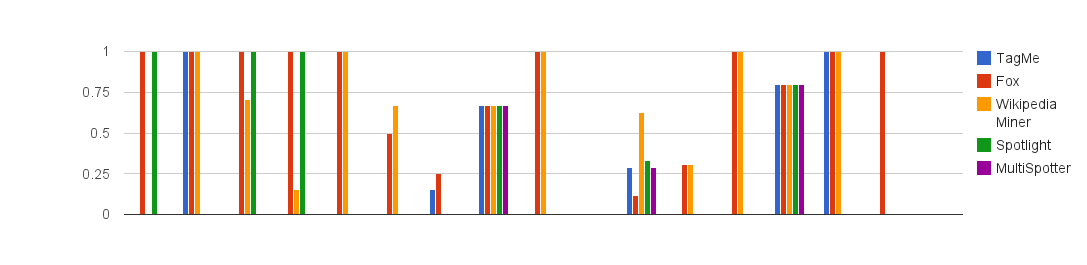
\includegraphics[width=\linewidth]{bars}
%\caption{Entity annotations systems performance with optimal ranking}
%\label{chahawk:fig:spiderOfEntityAnnotators}
%\end{figure}
%\footnote{Details on this evaluation can be found in the supplement on our project homepage.}


\subsection{Influence of Features while Ranking}
First, we evaluated the feature-based ranking method and its effectiveness and include an in-depth analysis of the contribution of each feature to the overall result.
Thus, we calculated the power set of the set of features and evaluated each feature group using the F-measure reached by the top-n queries. 
Figures~\ref{chahawk:fig:ranking_1} and ~\ref{chahawk:fig:ranking_2} show the F-measure@N for all query result sets of size $N$ from all 17 questions. 
%\todo[inline]{What exactly is shown in Figure 4 - i.e. there are F1/Precision/Recall scores for each of the 17 questions the system could answer, but how is the score calculated? I.e. either the systems get the right answer or not? Or is this based on top-N answers? Or based on how many correct answers from all the candidate queries?}
%\begin{minipage}{0.49\textwidth} 
%\centering
\begin{figure}[htb!]
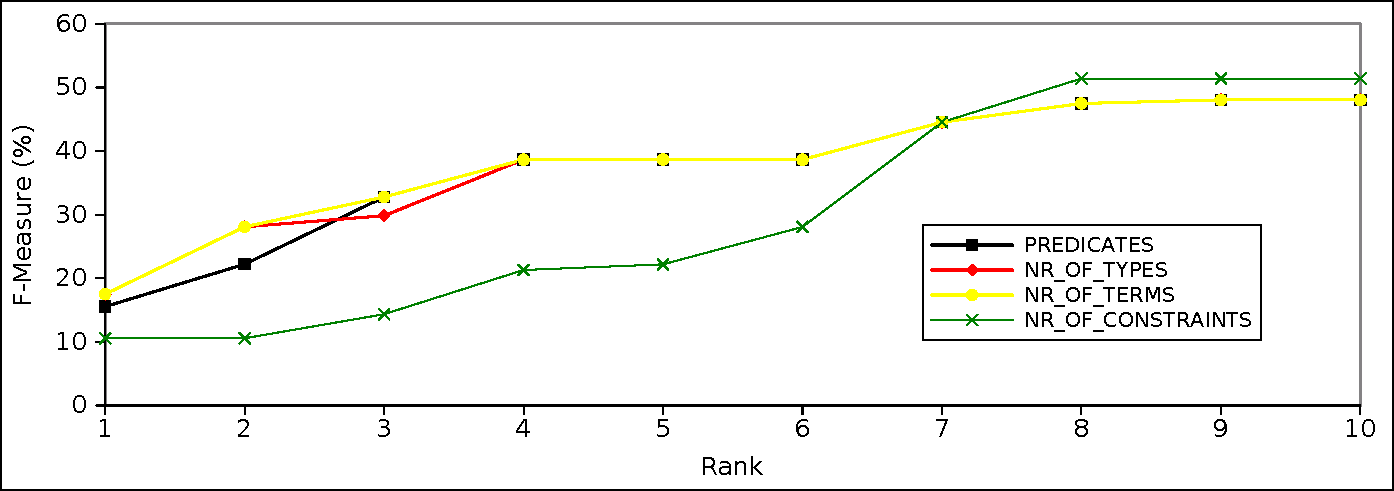
\includegraphics[width=\linewidth]{part_03/ESWC_HAWK/onefeature}
%\captionof{figure}{F-measures on training dataset using $N=[1,\ldots,10]$ and one feature.}
\caption{F-measures on training dataset using $N=[1,\ldots,10]$ and one feature.}
\label{chahawk:fig:ranking_1}
\end{figure}
%\end{minipage}
%\hfill
%\begin{minipage}{0.49\textwidth}
%\centering
\begin{figure}[htb!]
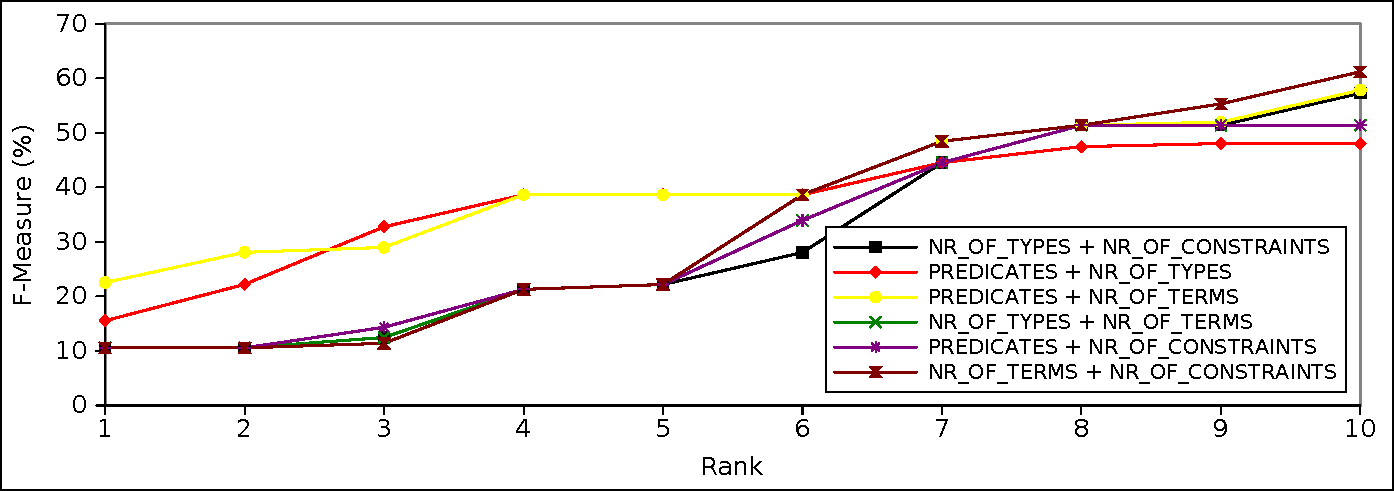
\includegraphics[width=\linewidth]{part_03/ESWC_HAWK/twofeature}
%\captionof{figure}{F-measures on training dataset using $N=[1,\ldots,10]$ and two features.}
\caption{F-measures on training dataset using $N=[1,\ldots,10]$ and two features.}
\label{chahawk:fig:ranking_2}
\end{figure}
%\end{minipage}

%\begin{minipage}{0.49\textwidth} 
%\centering
%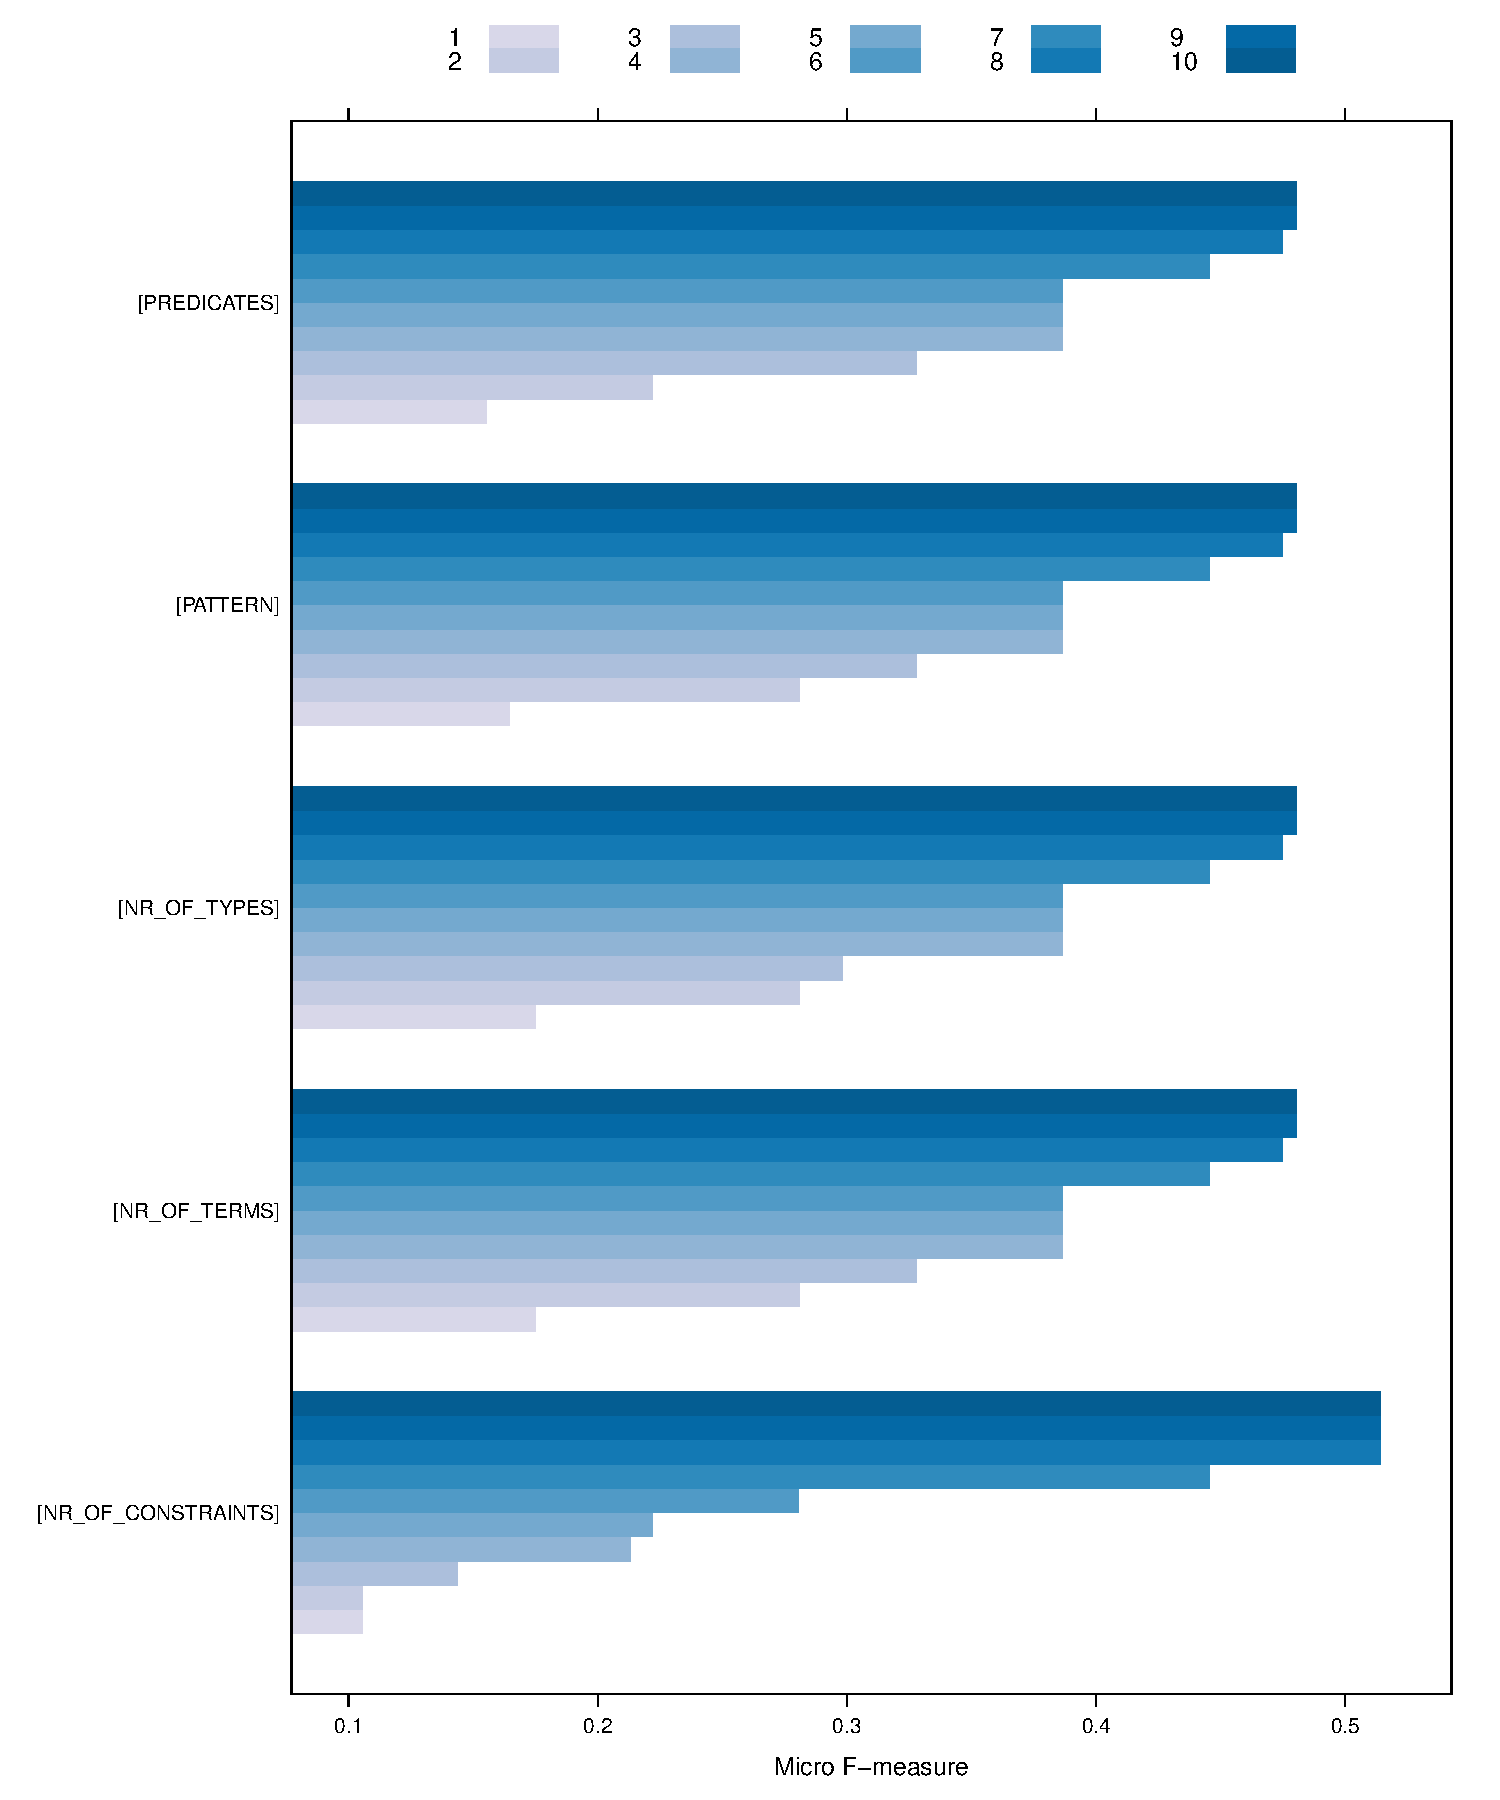
\includegraphics[width=\linewidth]{ranking_1}
%\captionof{figure}{F-measures on training dataset using $N=[1,\ldots,10]$ and one feature.}
%\label{chahawk:fig:ranking_1}
%\end{minipage}
%\hfill
%\begin{minipage}{0.49\textwidth}
%\centering
%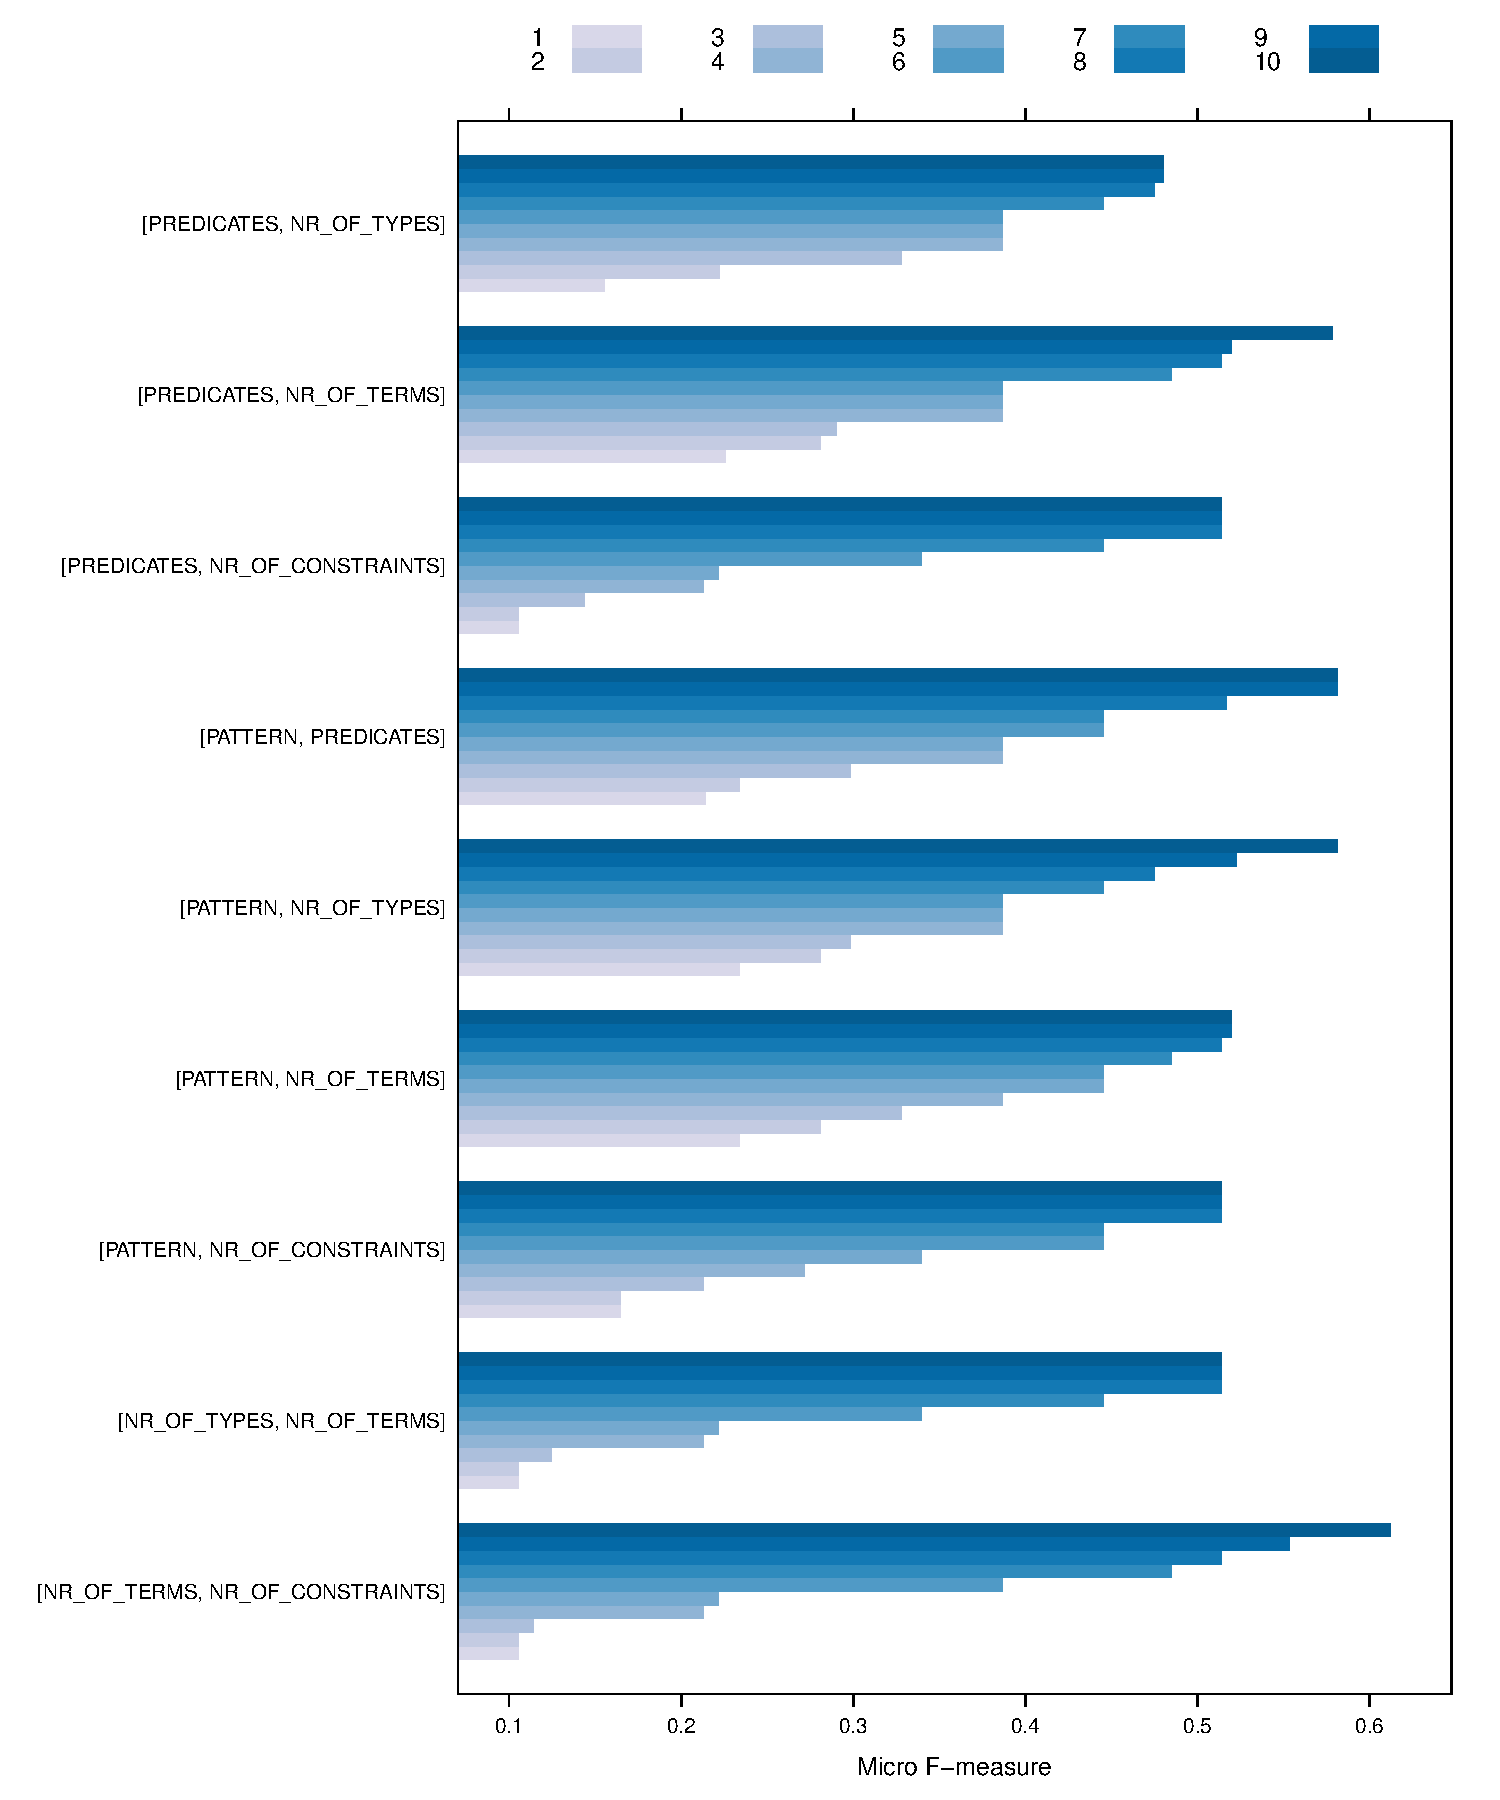
\includegraphics[width=\linewidth]{ranking_2}
%\captionof{figure}{F-measures on training dataset using $N=[1,\ldots,10]$ and two features.}
%\label{chahawk:fig:ranking_2}
%\end{minipage}

%\begin{minipage}{0.49\textwidth} 
%\centering
%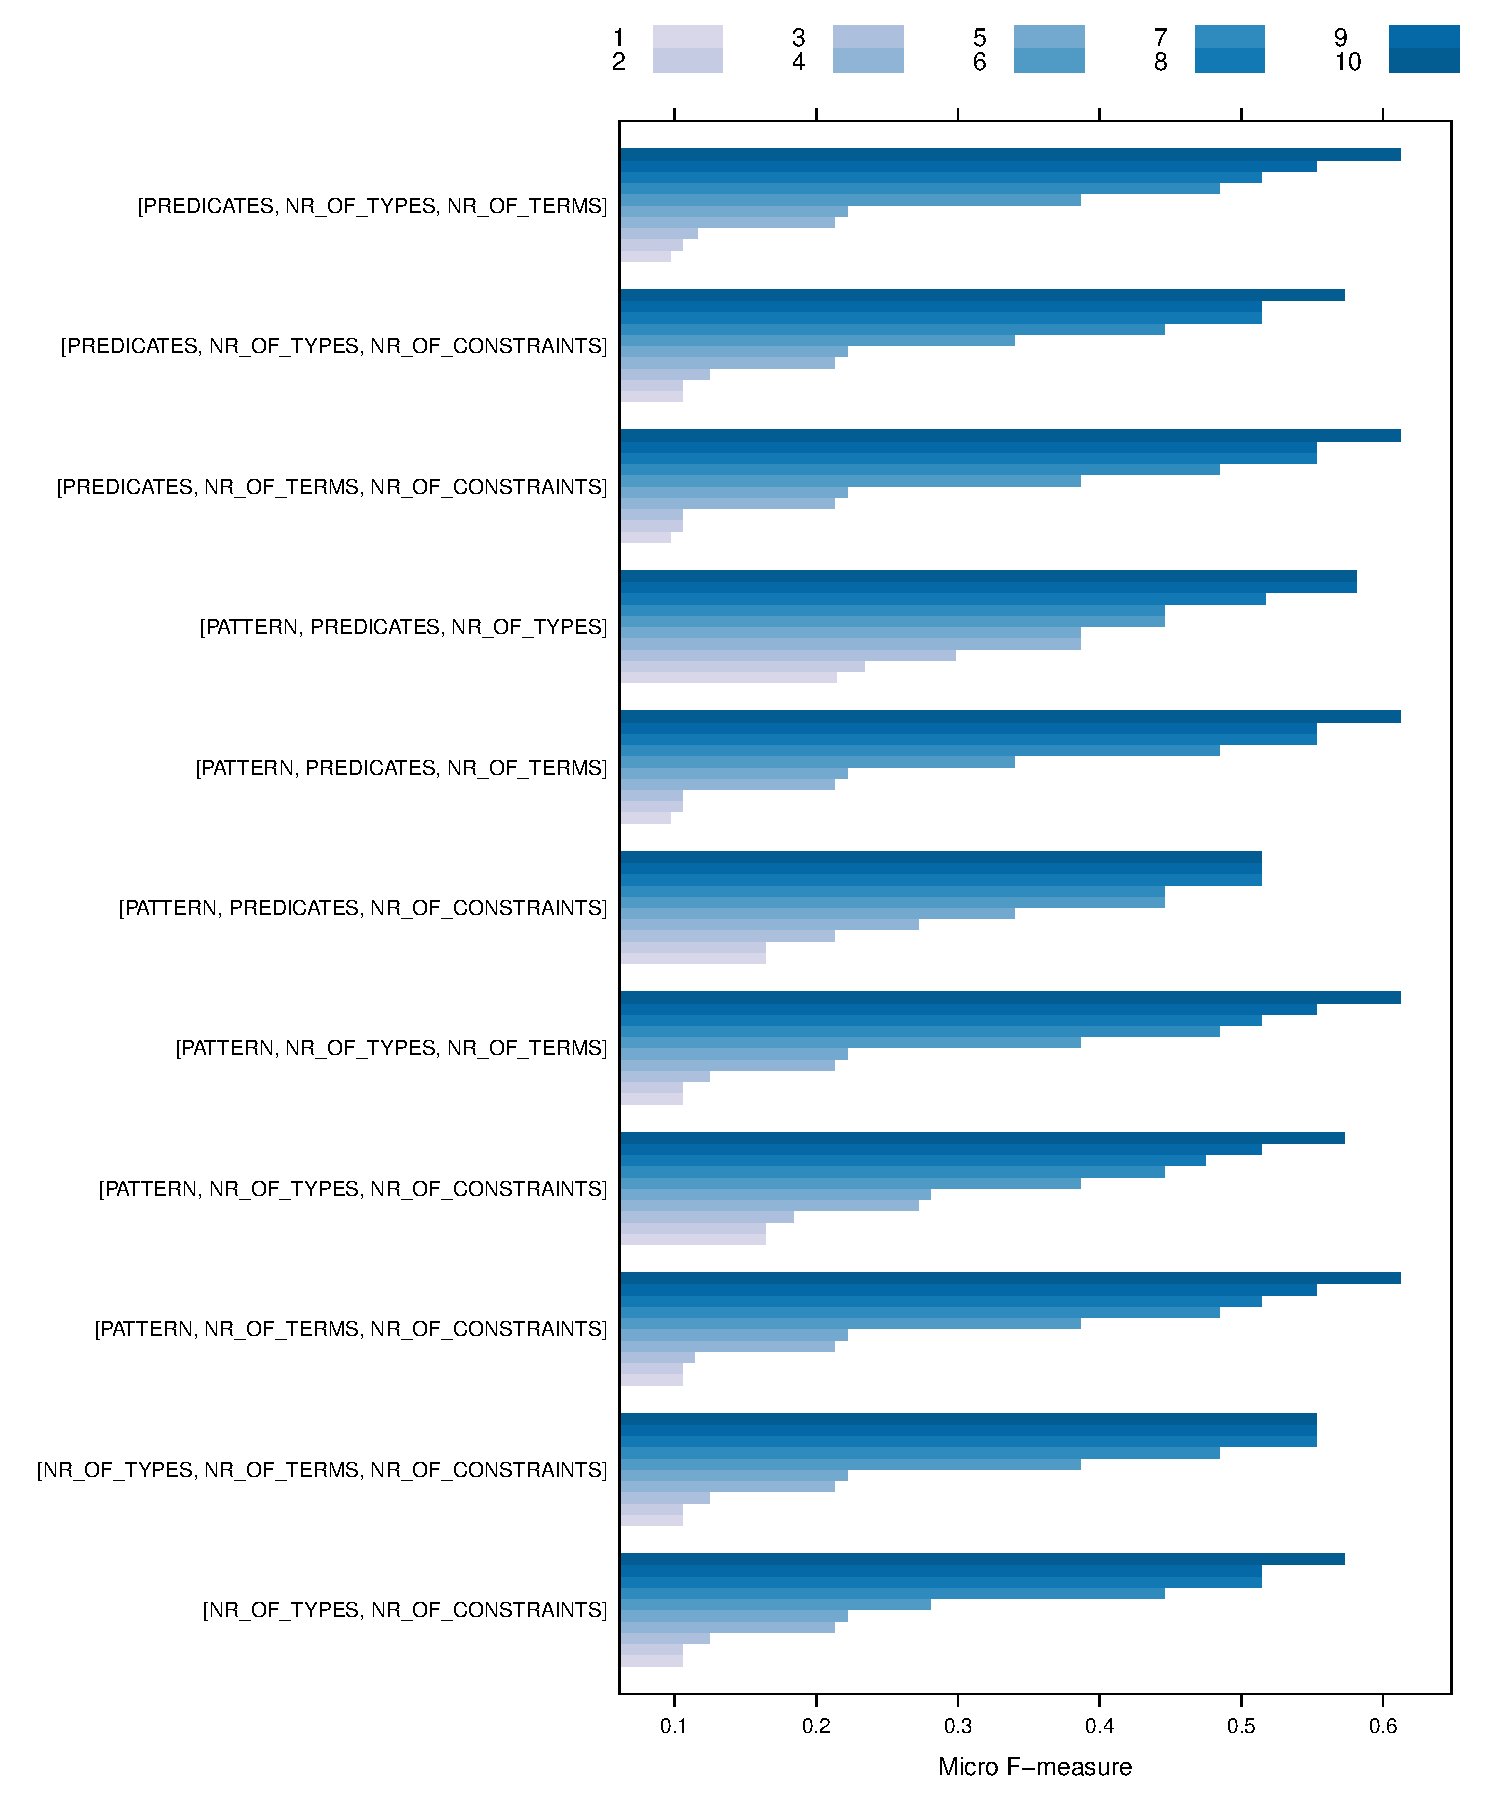
\includegraphics[width=\linewidth]{ranking_3}
%\captionof{figure}{F-measures on training dataset using $N=[1,\ldots,10]$ and three features.}
%\label{chahawk:fig:ranking_3}
%\end{minipage}
%\hfill
%\begin{minipage}{0.49\textwidth}
%\centering
%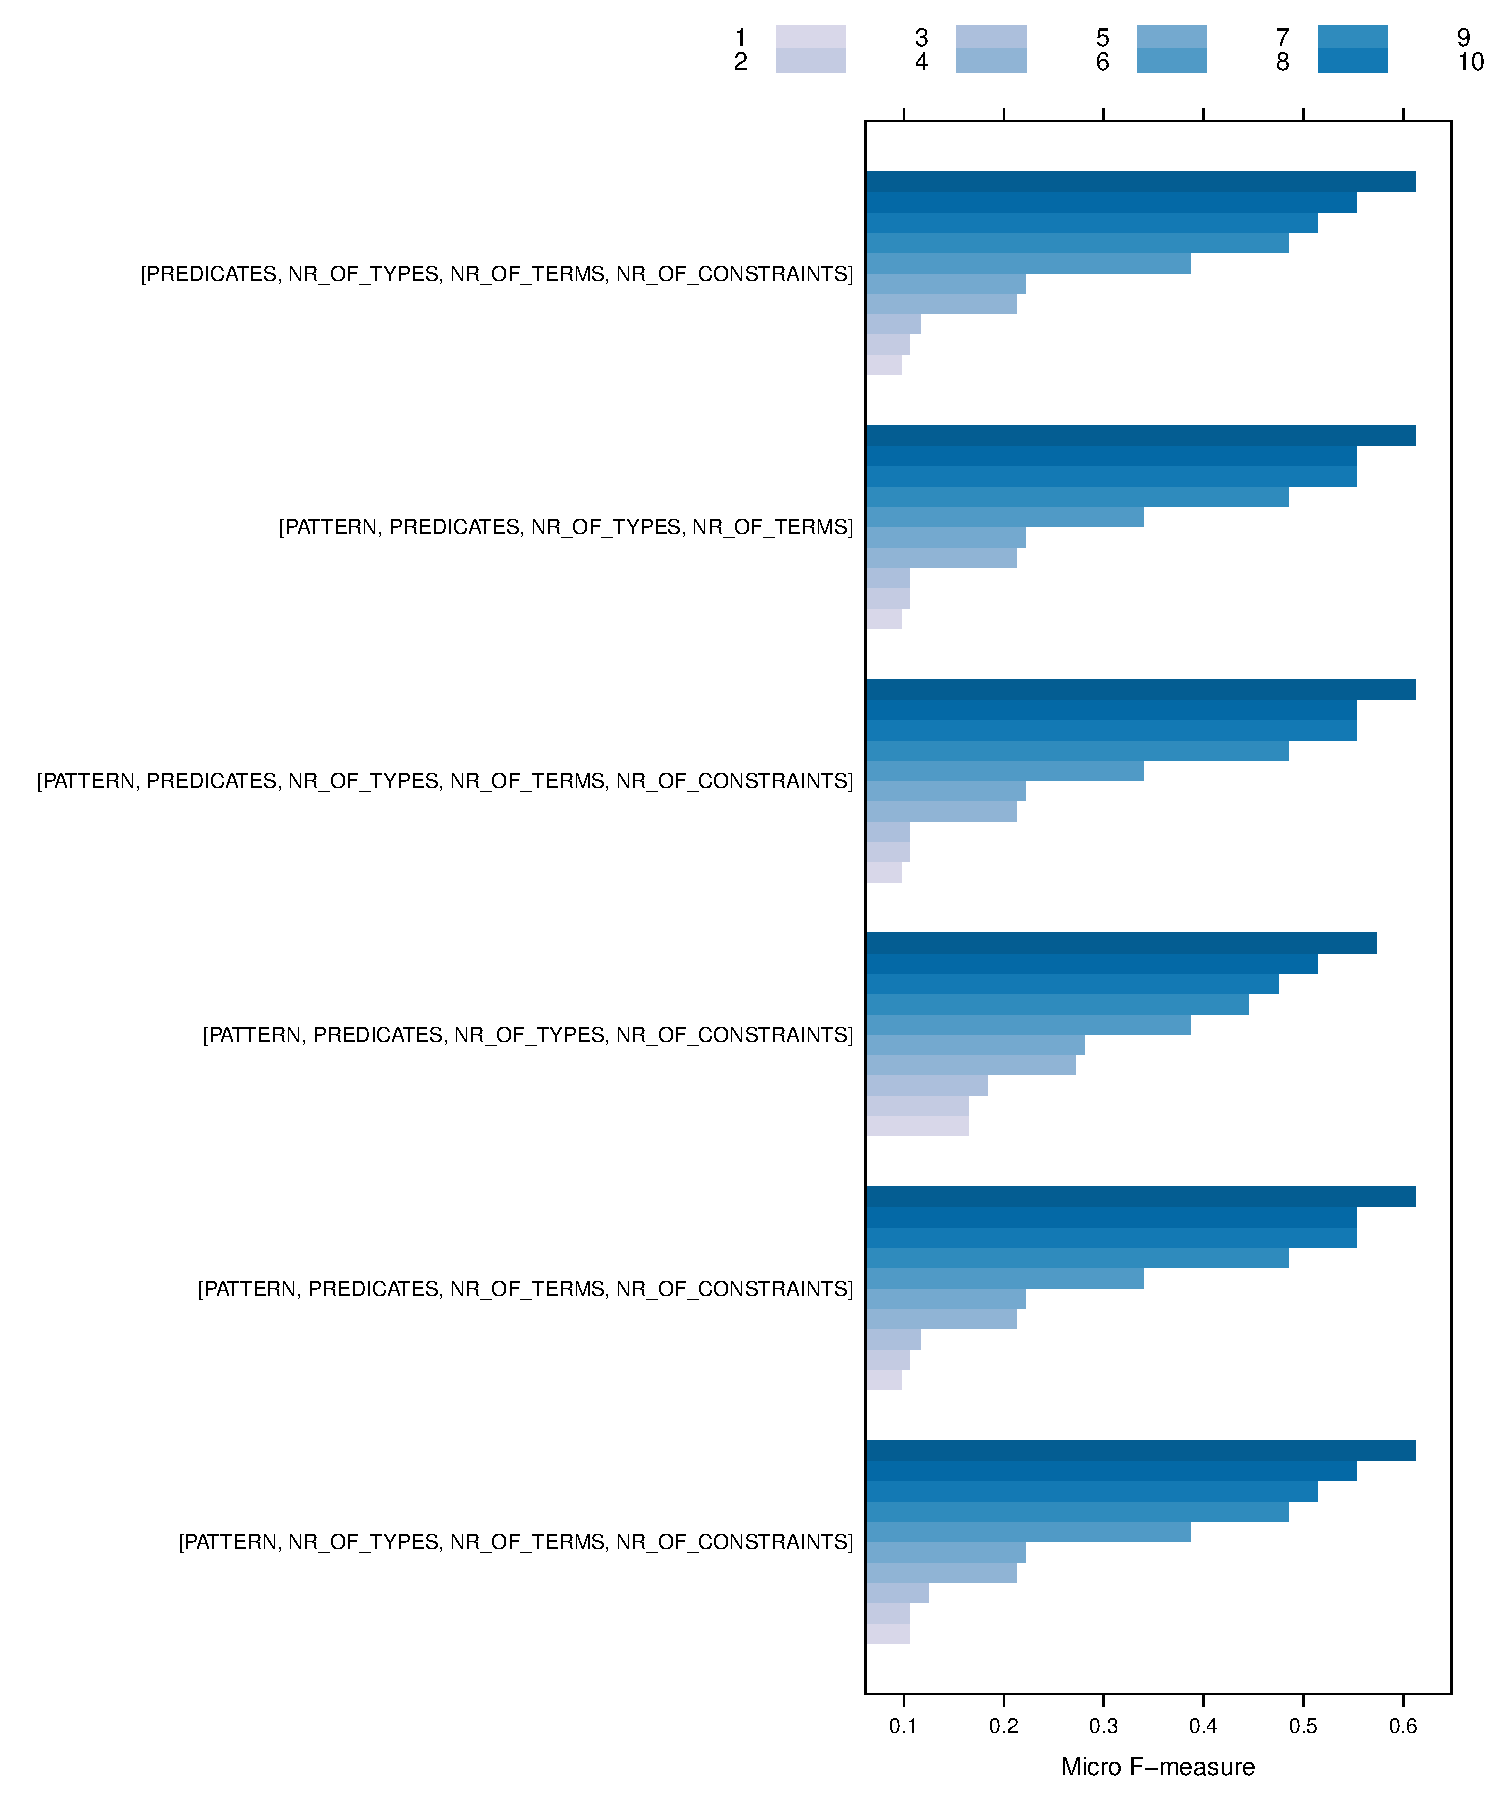
\includegraphics[width=\linewidth]{ranking_45}
%\captionof{figure}{F-measures on training dataset using $N=[1,\ldots,10]$ and using four and five features.}
%\label{chahawk:fig:ranking_45}
%\end{minipage}

Delving deeper into this analysis, we find:
\begin{itemize}
\item Although \textbf{NR\_OF\_TERMS} produces the largest sum of F-measures as a single feature, \textbf{NR\_OF\_CONSTRAINTS} achieves a higher F-measure as soon as $N=7$ due to the larger number of needed constraints with respect to the query length.
\item The highest F-measure reaches \textbf{PREDICATES, NR\_OF\_TERMS} with an F-measure of 0.58 at $N=10$. However, HAWK is able to achieve a higher F-measure of 0.61 at $N=10$ using \textbf{NR\_OF\_TERMS, NR\_OF\_CONSTRAINTS}.
\item We only regard the top-10-ranked queries. The correct queries belonged to the top-n queries as shown in Table~\ref{tab:trainqueries}.
\item The combination of three or all four features does not lead to an improvement. % of the F-measure. 
\end{itemize}

HAWK generates up to 15000 SPARQL queries per question containing more than one query generating the correct answer. 
We consider ranking the resulting SPARQL queries most challenging with respect to the fact that an ideal ranking can lead to F-measures up to 0.72 at $N=1$.



\section{Conclusion}
\label{chahawk:sec:conclusion}
\subsection*{Summary}
We introduced HAWK, a hybrid \ac{QA} system for the Web of Data and analyzed its performance against the combined \ac{QALD}-5 dataset using the new \texttt{ASK}-query module. 
We showed that by using a generic approach to generate SPARQL queries from predicate-argument structures, 
\begin{itemize}
\item HAWK is able to achieve up to 0.68 F-measure on the hybrid \ac{QALD}-4 benchmark using an optimal ranker.
\item The system is able to achieve an F-measure of up to 0.3 on the \ac{QALD}-5 training benchmark using bucket-based ranking.
\item Also, HAWK achieves a F-measure of up to 0.35 based on boolean and entiy-centric questions over the combined \ac{QALD}-5 benchmark.
\end{itemize}

\subsection*{Conclusion}
Currently, HAWK faces several limitations, such as not capturing the exact semantics due to missing dictionaries (e.g., vice-president), the ability to use \texttt{FILTER} and SPARQL aggregation functions (\texttt{FILTER (?high > 100)}) or compound questions. 
The most important open issue lies in finding the correct ranking approach to map a predicate-argument tree to a possible interpretation. 
So far, our experiments reveal that the mere finding of the right features for this endeavor remains a challenging problem. 

\subsection*{Future Work}
Currently, HAWK faces several limitations, such as not capturing the exact semantics due to missing dictionaries (e.g., vice-president), the ability to use \texttt{FILTER} and SPARQL aggregation functions (\texttt{FILTER (?high > 100)}) or compound questions. 
The most important open issue lies in finding the correct ranking approach to map a predicate-argument tree to a possible interpretation. 

Furthermore, we aim to integrate HAWK in domain-specific information systems where the more specialized context will most probably lead to higher F-measures. 
Additionally, we will assess the impact of full-text components over regular LD components for \ac{QA} and partake in the creation of larger benchmarks such as \ac{QALD}-6,
Another aim is to develop HAWK towards multilingual, schema-agnostic queries.
Also, negations within questions and improved ranking will also be considered. 
Finally, several components of the HAWK pipeline are computationally very complex. 
Thus, finding more time-efficient algorithms for these steps will be addressed in future works.
HAWK will be a starting point for the Eurostars projects DIESEL and QAMEL towards implementing novel search paradigms on large industrial data as well as mobile devices.
